%%%%%%%%%%%%%%%%%%%%%%%%%%%%%%%%%%%%%%%%%%%%%%%%%%%%%%%%%%%%%%%%%%%%%%%%%%%%%%%%
%
%
%
%%%%%%%%%%
\chapter{Evaluation}\label{ch:eval}


%%%%%%%%%%%%%%%%%%%%%%%%%%%%%%%%%%%%%%%%%%%%%%%%%%%%%%%%%%%%%%%%%%%%%%%%%%%%%%%%
%
%	- TODO: Stimmen die 10Hz?
%	- Start 13:50-23:50, 12:50-20:00 => 10+7 => 17 Stunden
%
%%%%%%%%%%
\section{Batterielaufzeit}

Beim Test der Batterielaufzeit wurden zwei \gls{uwbm} in einem Abstand von \SI{4.7}{\metre} aufgestellt. Beide \gls{uwbm} hatten eine direkte \gls{los} zu einandern. Über den kompletten Zeitraum wurden Entfernungsmessungen mit einer Rate von \SI{10}{\hertz} durchgeführt. Als Testprogramme wurden dabei \textit{DW1000Ranging\_ANCHOR} und \textit{DW1000Ranging\_TAG} aus dem GitHub-Projekt \cite{Trojer2015} verwendet.

Der \Gls{anchor} hatte nach ca. \SI{17}{\hour} seinen Dienst eingestellt, wenig später folgte Ihm der \Gls{tag}. Deutlich höhere Batterielaufzeiten können dadurch erzielt werden, dass die Senderate reduziert wird und die Stromsparfunktionen sowohl des DWM1000 als auch des ATmega328/P genutzt werden.


%%%%%%%%%%%%%%%%%%%%%%%%%%%%%%%%%%%%%%%%%%%%%%%%%%%%%%%%%%%%%%%%%%%%%%%%%%%%%%%%
%
%	- 3-sigma
%		- https://www.easycalculation.com/statistics/learn-three-sigma.php
%		- https://bizfluent.com/how-5214886-calculate-sigma.html
%		- https://stackoverflow.com/questions/28699342/calculate-the-3rd-standard-deviation-for-an-array
%
%%%%%%%%%%
\section{Kalibierung}

Um die Antennenverzögerung pro \Gls{uwbm} zu bestimmen, werden zwei Kalibriervorgänge durchgeführt. Der erste Kalibriervorgang orientiert sich an den Herstellervorgaben aus \cite{decawave2014calibration}. Dazu werden drei \Glspl{uwbm} an die Spitzen eines gleichseitigen Dreieckes positioniert. Um das Dreieck zu konstruieren, wird in der Mitte des Dreiecks eine ausgemessene Maurerschnur befestigt, darüber wird eine Winkelschablone gelegt und dann reihum die Spitzen es Dreiecks auf dem Boden eingezeichnet, siehe \autoref{fig:calibration_triangle2}. Die Seitenlänge $a \approx \SI{1.73}{\meter}$ wird dabei aus dem Umkreisradius $r_u = \SI{1}{\meter}$ mit der \autoref{eq:dreieck_seitenlaenge_aus_umkreis} berechnet.

\begin{figure}[h]
	\centering
	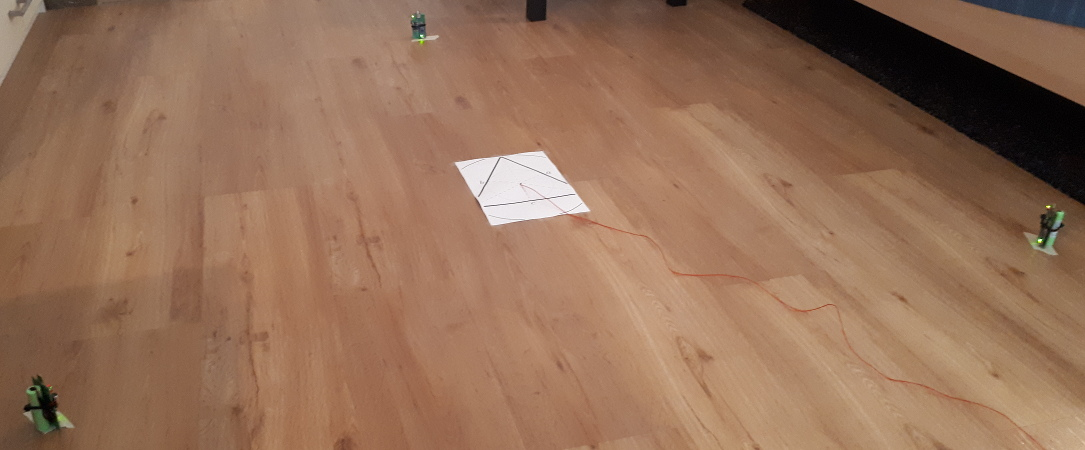
\includegraphics[width=0.9\linewidth]{calibration_triangle2}
	\caption{Versuchsaufbau für die Kalibierung von drei \Glsuseri{uwbm}.}
	\label{fig:calibration_triangle2}
\end{figure}

Initial wird die Antennenverzögerung bei allen \Glsuseri{uwbm} auf null gesetzt und danach reihum von jedem \Gls{uwbm} eintausend Entfernungsmessungen zu den beiden benachbarten \Glsuseri{uwbm} durchgeführt. Insgesamt entstehen dabei sechstausend Datensätze, die mittels dem \textit{LGS}- bzw. des \textit{DecaWave}-Kalibrierungsverfahren ausgewertet werden, siehe \autoref{tab:calibration_antenna_delay_results}

Das \textit{LGS}-Kalibrierungsverfahren lieferte für jeden Durchlauf reproduzierbare Ergebnisse. Da jedes \Gls{uwbm} herstellungsbedingte Unterschiede aufweist, ist es Plausibel das alle Antennenverzögerungen in einem ähnlichen Wertebereich liegen. Anders sieht es bei dem \textit{DecaWave}-Kalibrierungsverfahren aus. Hier ergeben sich für jeden Durchlauf andere Wertekombinationen, bedingt durch die Zufallskomponente bei der Erstellung der Kandidatenliste. Diese Verhalten von Genetischen-Algorithmen ist bekannt und muss daher bei der Auswahl der Wertekombinationen berücksichtigt werden. Am Beispiel der Spalte \textit{DecaWave 1} wird es sehr deutlich. Hier beträgt der Unterschied zwischen dem größten und kleinsten Wert \approx\SI{23}{\ns} und entspricht damit einer Abweichung von \approx\SI{6}{\meter} zwischen diesen beiden \Glsuseri{uwbm}.

% todo: Im Text ist von Nanosekunden die Rede, in der Tabelle aber von Sekunden.
\begin{table}[h]
	\centering
	\begin{tabular}{||c||c||ccc||}
\hline
\Gls{uwbm} & LGS & DecaWave & DecaWave 1 & DecaWave 2 \\
& [\si{\nano\second}] & [\si{\nano\second}] & [\si{\nano\second}] & [\si{\nano\second}] \\
\hline
\hline
176 & \num{257.45} & \num{242.48} & \num{232.21} & \num{254.50} \\
177 & \num{257.49} & \num{238.47} & \num{249.38} & \num{254.73} \\
178 & \num{257.11} & \num{257.17} & \num{255.36} & \num{215.07} \\
\hline
% Alte Darstellung
%176 & 16451 & 15494 & 14838 & 15912 & 16262 \\
%177 & 16453 & 15238 & 15935 & 15805 & 16277 \\
%178 & 16429 & 16433 & 16317 & 15131 & 13743 \\
	\end{tabular}
	\caption{Berechnete Werte für die Antennenverzögerung pro \glsentryshort{uwbm}.}
	\label{tab:calibration_antenna_delay_results}
\end{table}

Die Wertekombinationen aus den Spalten \textit{LGS} und \textit{DecaWave} werden abwechselnd als Antennenverzögerungen in die \Glspl{uwbm} eingetragen und für jede Spalte jeweils eine weitere Messreihe, wie oben beschrieben, aufgezeichnet. Die Ergebnisse sind in der \autoref{tab:calibration_range_results} aufgeführt.

Mit einer initalen Antennenverzögerung von null beträgt die gemessene Entfernung zwischen zwei \Glsuseri{uwbm} \approx \SI{156}{\meter} bei einer tatsächenlichen Entfernung von \approx \SI{1.73}{\meter}. Eine Standardabweichung von \approx \SI{2}{\centi\meter} \footnote{Bei der Standardabweichung von über einem Meter handelt es sich um einen einzelnen Messfehler in der Messreihe.} entspricht dabei den Produkteigenschaften mit denen \textit{DecaWave} wirbt.

Werden die Antennenverzögerung aus der \textit{LGS}-Kalibrierungsverfahren benutzt, verbleibt die Standardabweichung in der gleichen Größenordnung wie im unkalibrierten Zustand. Jedoch nähert sich jetzt die gemessenen Entfernungen der tatsächlichen sehr stark an und bildet diesen sehr gut ab. Ganz im Gegensatz zu dem \textit{DecaWave}-Ka\-li\-brierungs\-ver\-fahren.

\begin{table}[h]
	\centering
	\begin{tabular}{||c||cc||ccc|cc||}
\hline
Kalibrierung & Tag & Anker & Entfernung & $\overline{x}$ & $\sigma$ & Min & Max \\
 & & & [\si{\meter}] & [\si{\meter}] & [\si{\meter}] & [\si{\meter}] & [\si{\meter}] \\
\hline
\hline
Keine & 176 & 177 & \num{1.732} & \num{156.108} & \num{0.018} & \num{156.050} & \num{156.170} \\
Keine & 176 & 178 & \num{1.732} & \num{155.929} & \num{0.021} & \num{155.870} & \num{156.000} \\
Keine & 177 & 176 & \num{1.732} & \num{156.106} & \num{1.025} & \num{156.020} & \num{188.470} \\
Keine & 177 & 178 & \num{1.732} & \num{156.016} & \num{0.023} & \num{155.930} & \num{156.090} \\
Keine & 178 & 176 & \num{1.732} & \num{156.067} & \num{0.022} & \num{156.010} & \num{156.130} \\
Keine & 178 & 177 & \num{1.732} & \num{155.997} & \num{0.019} & \num{155.930} & \num{156.060} \\
\hline
LGS & 176 & 177 & \num{1.732} & \num{1.695} & \num{0.019} & \num{1.640} & \num{1.750} \\
LGS & 176 & 178 & \num{1.732} & \num{1.795} & \num{0.022} & \num{1.740} & \num{1.880} \\
LGS & 177 & 176 & \num{1.732} & \num{1.656} & \num{0.017} & \num{1.590} & \num{1.700} \\
LGS & 177 & 178 & \num{1.732} & \num{1.751} & \num{0.023} & \num{1.670} & \num{1.810} \\
LGS & 178 & 176 & \num{1.732} & \num{1.773} & \num{0.026} & \num{1.700} & \num{1.850} \\
LGS & 178 & 177 & \num{1.732} & \num{1.712} & \num{0.020} & \num{1.660} & \num{1.780} \\
\hline
DecaWave & 176 & 177 & \num{1.732} & \num{11.883} & \num{0.020} & \num{11.820} & \num{11.950} \\
DecaWave & 176 & 178 & \num{1.732} & \num{6.261} & \num{0.021} & \num{6.200} & \num{6.340} \\
DecaWave & 177 & 176 & \num{1.732} & \num{11.857} & \num{0.015} & \num{11.810} & \num{11.900} \\
DecaWave & 177 & 178 & \num{1.732} & \num{7.406} & \num{0.023} & \num{7.340} & \num{7.480} \\
DecaWave & 178 & 176 & \num{1.732} & \num{6.182} & \num{0.025} & \num{6.100} & \num{6.270} \\
DecaWave & 178 & 177 & \num{1.732} & \num{7.458} & \num{0.019} & \num{7.390} & \num{7.520} \\
\hline
	\end{tabular}
	\caption{Stochastische Eigenschaften der \Glspl{uwbm} ohne und mit Antennenkalibrierung bei einem Abstand von \SI{1.73}{\meter}.}
	\label{tab:calibration_range_results}
\end{table}

In der \autoref{fig:calibration_histograms} wurden die gemessenen Entfernungen als Histogramm dargestellt. Gut zu erkennen ist die Normalverteilung der Messwerte um den Mittelwert.

\begin{figure}[h]
	\centering
	\begin{subfigure}[b]{0.32\linewidth}
		\centering
		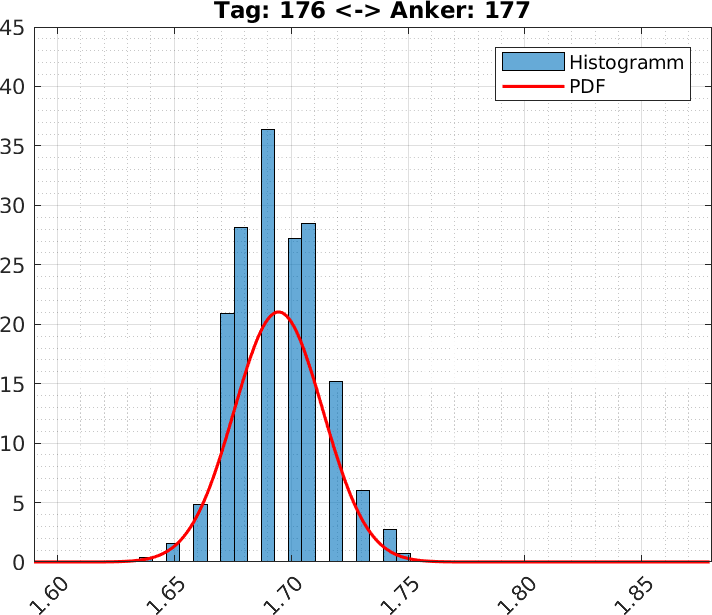
\includegraphics[width=\linewidth]{calibration_histogram_176_177}
	\end{subfigure}
	\hfill
	\begin{subfigure}[b]{0.32\linewidth}
		\centering
		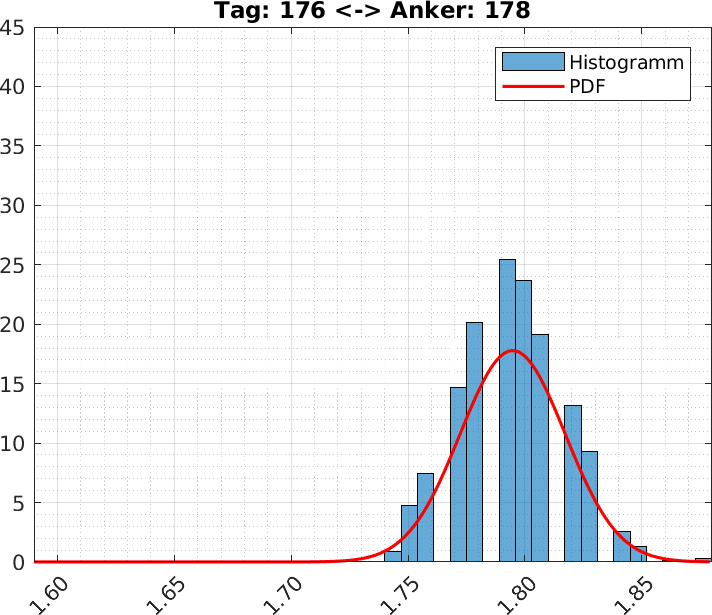
\includegraphics[width=\linewidth]{calibration_histogram_176_178}
	\end{subfigure}
	\hfill
	\begin{subfigure}[b]{0.32\linewidth}
		\centering
		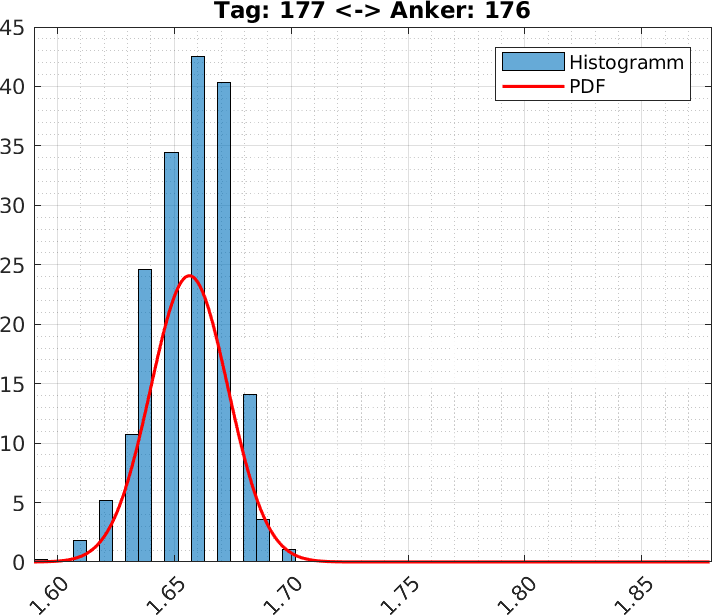
\includegraphics[width=\linewidth]{calibration_histogram_177_176}
	\end{subfigure}
	\par
	\bigskip
	\begin{subfigure}[b]{0.32\linewidth}
		\centering
		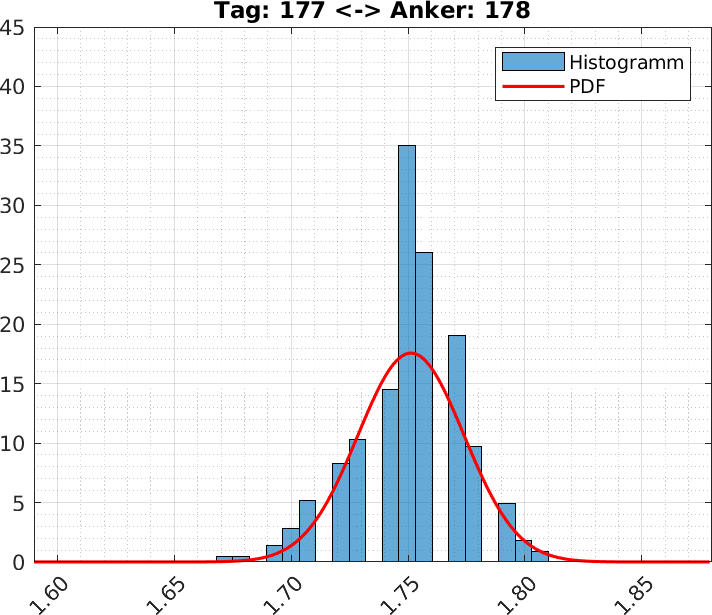
\includegraphics[width=\linewidth]{calibration_histogram_177_178}
	\end{subfigure}
	\hfill
	\begin{subfigure}[b]{0.32\linewidth}
		\centering
		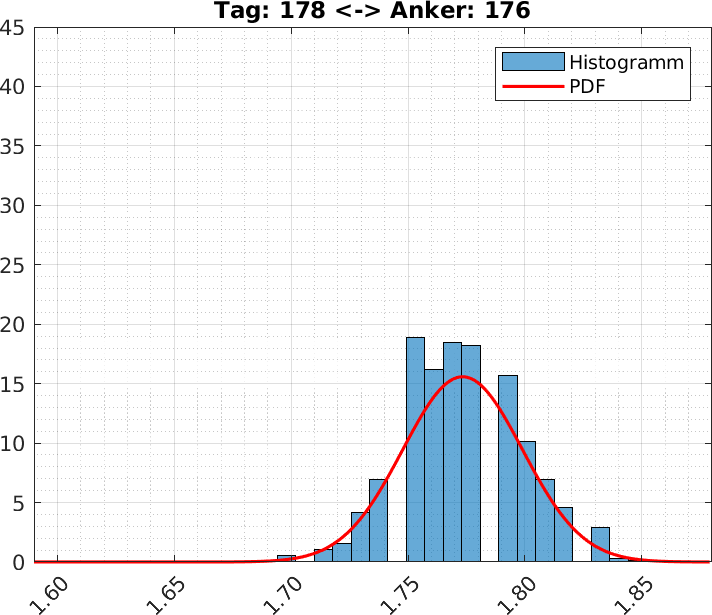
\includegraphics[width=\linewidth]{calibration_histogram_178_176}
	\end{subfigure}
	\hfill
	\begin{subfigure}[b]{0.32\linewidth}
		\centering
		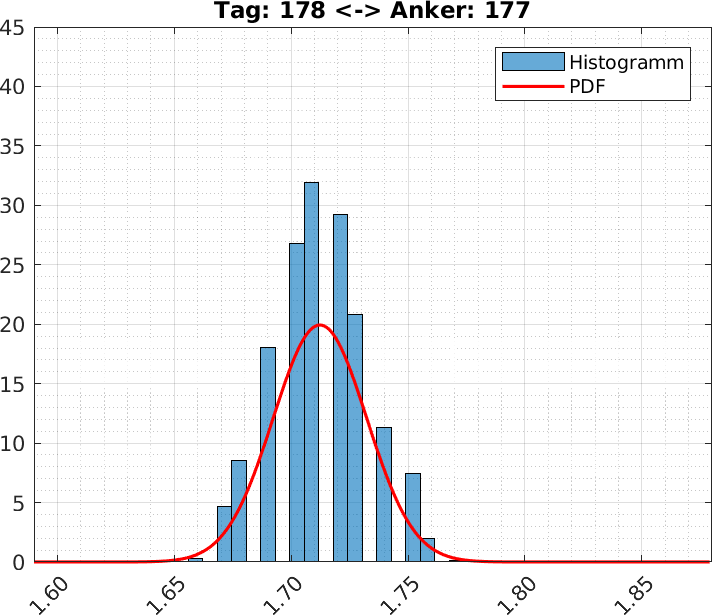
\includegraphics[width=\linewidth]{calibration_histogram_178_177}
	\end{subfigure}
	\caption{Histogramm und Wahrscheinlichkeitsdichtefunktion der kalibrierten Entfernungsmessungen.}
	\label{fig:calibration_histograms}
\end{figure}

Im zweiten Kalibriervorgang werden alle fünf \Glspl{uwbm} eingeschlossen. Jetzt reicht ein Dreieck nicht mehr aus, statt dessen wird ein regelmäßiges Fünfeck/Pentagramm verwendet, siehe \autoref{fig:calibration_pentagram2}. Dieses lässt sich mathematisch ähnlich gut beschreiben wie das Dreieck. Aus der Seitenlänge $a = \SI{4.5}{\meter}$, zwischen zwei benachbarten Spitzen, wird über die \autoref{eq:fuenfeck_diagonale} die Entfernung $d$, zwischen den diagonalen Spitzen, berechnet. Der Umkreisradius $r_u$ ergibt sich aus der \autoref{eq:fuenfeck_umkreisradius}.

\begin{figure}[h]
	\centering
	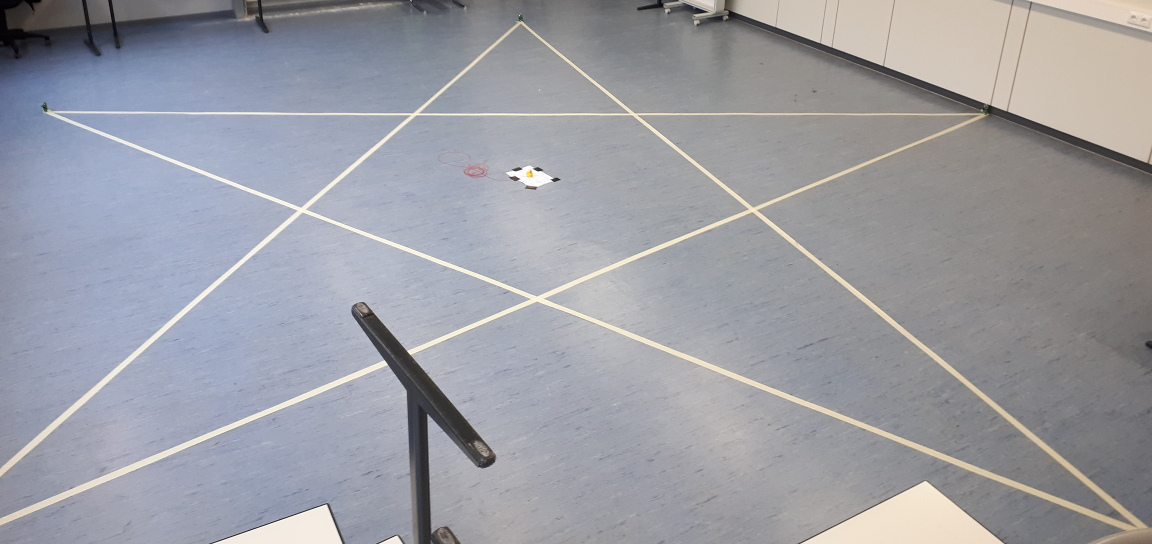
\includegraphics[width=0.9\linewidth]{calibration_pentagram2}
	\caption{Versuchsaufbau für die Kalibierung von fünf \glsuseri{uwbm}.}
	\label{fig:calibration_pentagram2}
\end{figure}

Für das regelmäßige Fünfeck/Pentagramm wurde nur noch das \textit{LGS}-Ka\-li\-brie\-rungs\-ver\-fahren verwendet, die Antennenverzögerungen pro \Gls{uwbm} sind dabei in der \autoref{tab:calibration_pentagramm_antenna_delay_results} aufgeführt.

\begin{table}[h]
	\centering
	\begin{tabular}{||c||c||}
\hline
\Gls{uwbm} & LGS \\
 & [\si{\nano\second}] \\
\hline\hline
176 & \num{257.30} \\
177 & \num{256.67} \\
178 & \num{256.67} \\
179 & \num{256.41} \\
180 & \num{257.20} \\

% Alte Darstellung
%176 & 16441 \\
%177 & 16401 \\
%178 & 16401 \\
%179 & 16384 \\
%180 & 16435 \\
\hline
	\end{tabular}
	\caption{Berechnete Werte für die Antennenverzögerung pro \glsentryshort{uwbm} für das regelmäßige Fünfeck/Pentagramm.}
	\label{tab:calibration_pentagramm_antenna_delay_results}
\end{table}


%%%%%%%%%%%%%%%%%%%%%%%%%%%%%%%%%%%%%%%%%%%%%%%%%%%%%%%%%%%%%%%%%%%%%%%%%%%%%%%%
%
%	- Wie verändert sich die Genauigkeit der Entfernungsmessung bei einer direkten Sichtverbindung (engl. Line-of-sight (LOS)) und indirekten Sichtverbindung (engl. Non-line-of-sight (NLOS))?
%	- Stochastik
%		- https://matheguru.com/stochastik/mittel-durchschnitt-und-lageparameter.html
%		- https://matheguru.com/stochastik/standardabweichung.html
%		- https://matheguru.com/stochastik/standardfehler.html

%
%%%%%%%%%%
\section{Entfernungsmessung}

Um die Charakteristik der Entfernungsmessung zu bestimmen, wird eine \Gls{los}- und drei \Gls{nlos}-Messreihen aufgezeichnet. Jede Messreihe beginnt bei einer Entfernung von einem Meter zwischen \Gls{tag} und \Gls{anchor}. Pro Entfernung werden jeweils fünfhundert Messwerte aufgezeichnet. Danach wird die Entfernung um einen halben Meter erhöht, indem der \Gls{anchor} verschoben wird. Dies erfolgt solange bis eine Entfernung von neun Meter erreicht ist. Somit enthält jede Messreihe siebzehn Entfernungen mit achttausendfünfhundert Entfernungsmessungen.

Bei der ersten \Gls{nlos}-Messreihe wird ein \SI{19x12x10}{\centi\meter} großer, mit Wasser gefüllter Kunststoffbehälter in einem Abstand von \SI{2}{\centi\meter} vor der \Gls{uwb}-Antenne platziert, siehe \autoref{fig:entfernungsmessung_versuchsaufbau_20180120_133013}. Bei den letzten zwei \Gls{nlos}-Messreihen wird ein \SI{44x25}{\centi\meter} großes Aluminiumblech mit einer Dicke von \SI{0.5}{\milli\meter} vor die \Gls{uwb}-Antenne platziert, jeweils in einem Abstand von \SI{5}{\centi\meter} und \SI{50}{\centi\meter}, siehe \autoref{fig:entfernungsmessung_versuchsaufbau_20180120_140118} und \autoref{fig:entfernungsmessung_versuchsaufbau_20180120_122434}.


\begin{figure}[ht]
	\begin{minipage}{0.49\linewidth}
		\begin{subfigure}{\linewidth}
			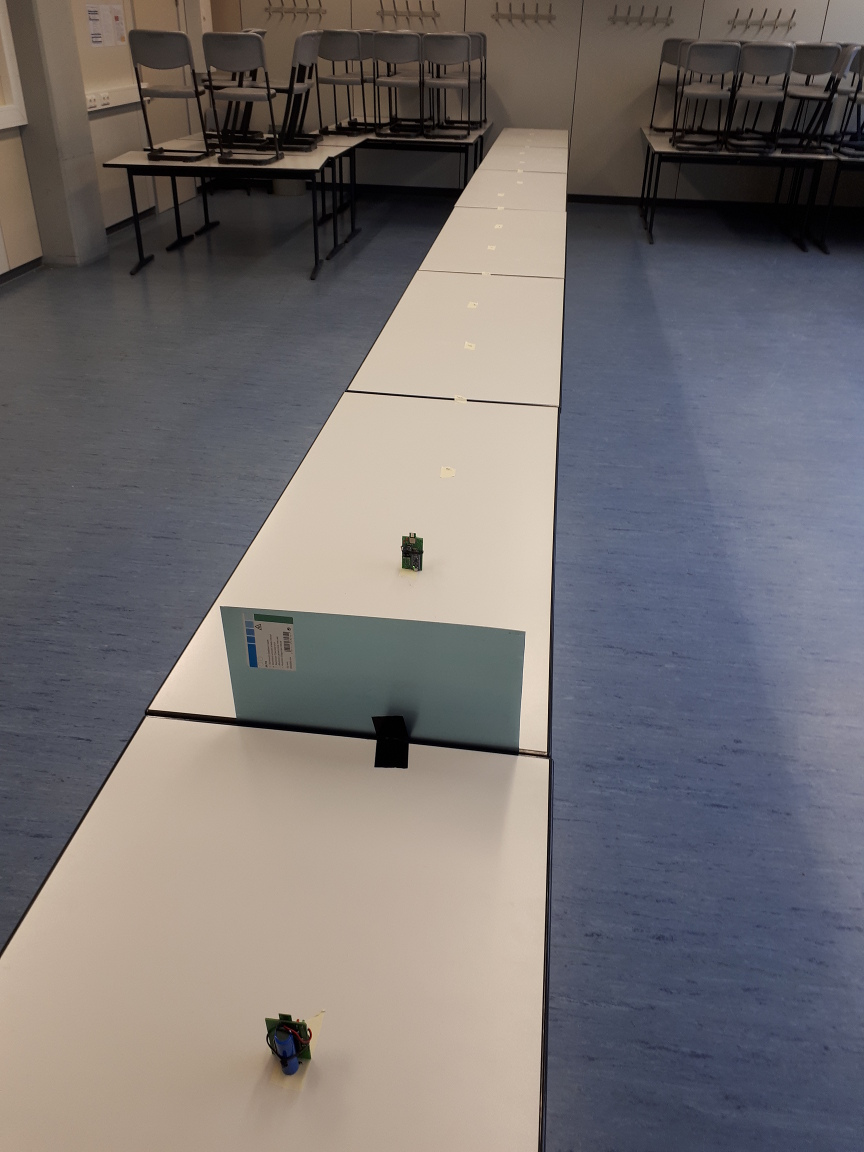
\includegraphics[width=\linewidth]{entfernungsmessung_versuchsaufbau_20180120_122434_2}
			\caption{ }
			\label{fig:entfernungsmessung_versuchsaufbau_20180120_122434}
		\end{subfigure}
	\end{minipage}
	\hfill
	\begin{minipage}{0.49\linewidth}
			\begin{minipage}{\linewidth}
				\begin{subfigure}{\linewidth}
					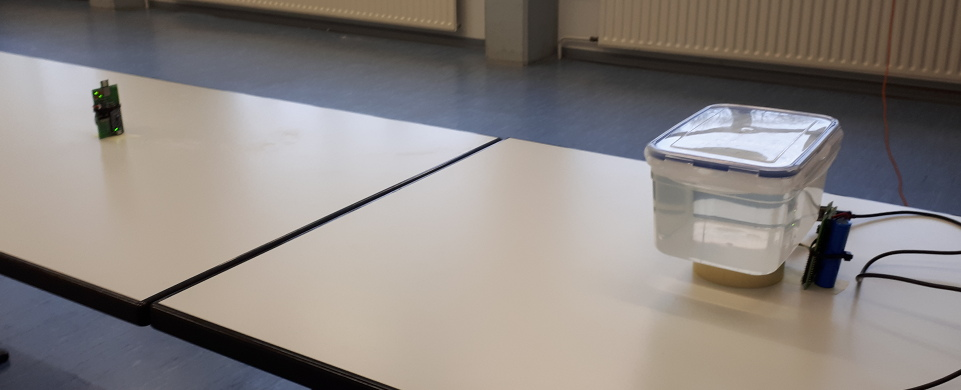
\includegraphics[width=\linewidth]{entfernungsmessung_versuchsaufbau_20180120_133013_2}
					\caption{ }
					\label{fig:entfernungsmessung_versuchsaufbau_20180120_133013}
				\end{subfigure}
			\end{minipage}
			\par
			\bigskip
			\begin{minipage}{\linewidth}
				\begin{subfigure}{\linewidth}
					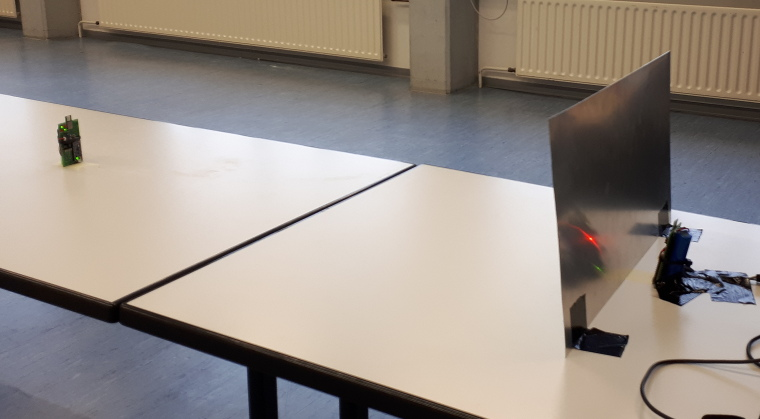
\includegraphics[width=\linewidth]{entfernungsmessung_versuchsaufbau_20180120_140118_2}
					\caption{ }
					\label{fig:entfernungsmessung_versuchsaufbau_20180120_140118}
				\end{subfigure}	
			\end{minipage}
	\end{minipage}
	\caption{Versuchsaufbau für die \glsentryshort{nlos}-Entfernungsmessung.}
	\label{fig:entfernungsmessung_versuchsaufbau_20180120}
\end{figure}


Das auffälligste Merkmal der \Gls{los}- als auch der \Gls{nlos}-Entfernungsmessungen ist die systematische Verschiebung aller Messwerte um ca. \SI{20}{\centi\meter} deren Ursache ungeklärt bleibt, siehe \autoref{fig:entfernungsmessung_2018_01_20}.

Bei der \Gls{los}-Messreihe beträgt die Standardabweichung, wie bereits bei der Kalibrierung, ca. \SI{2}{\centi\meter}. Mit steigender Entfernung steigt auch die Standardabweichung von ca. \SI{1.8}{\centi\meter} bei einem Meter auf ca. \SI{2.3}{\centi\meter} bei neun Meter an. Größere Ausreißer sind bei den Messwerten nicht vorhanden, siehe \autoref{fig:entfernungsmessung_2018_01_20_los} und \autoref{tab:entfernungsmessung_2018_01_20_los}.

In der \autoref{fig:entfernungsmessung_2018_01_20_nlos_water} ist deutlich zu erkennen, das Wasser einen sehr störenden Einfluss auf die Entfernungsmessung ausübt. Die Messwerte streuen über einen sehr großen Bereich, das spiegelt sich auch in der Standardabweichung, die im besten Fall ca. \SI{5}{\centi\meter} und im schlimmsten Fall ca. \SI{34}{\centi\meter} beträgt, siehe \autoref{tab:entfernungsmessung_2018_01_20_nlos_water}.

Ähnlich verhält es sich bei der \Gls{nlos}-Messreihe mit einem Aluminiumblech, das sehr nah vor der \Gls{uwb}-Antenne platziert wurde, siehe \autoref{fig:entfernungsmessung_2018_01_20_nlos_metal2} und \autoref{tab:entfernungsmessung_2018_01_20_nlos_metal2}. Einzig im Bereich von zwei bis fünf Meter beträgt die Standardabweichung ca. \SI{2}{\centi\meter}.

Keinen besonders großen Einfluss hat das Aluminiumblech, wenn es sich in einer Entfernung von \SI{50}{\centi\meter} befindet, siehe \autoref{tab:entfernungsmessung_2018_01_20_nlos_metal}. Die Werte der Standardabweichung ähneln der \Gls{los}-Messreihe. Nur im Bereich zwischen achteinhalb und neun Meter steigt die Standardabweichung auf einen Wert von ca. \SI{30}{\centi\meter} an. Dies könnte darauf zurückzuführen sein, das im hinteren Bereich des Raums Metallstühle auf den Tischen standen, siehe \autoref{fig:entfernungsmessung_versuchsaufbau_20180120_122434}.


\begin{figure}[ht]
	\centering
	\begin{subfigure}[t]{0.49\linewidth}
		\centering
		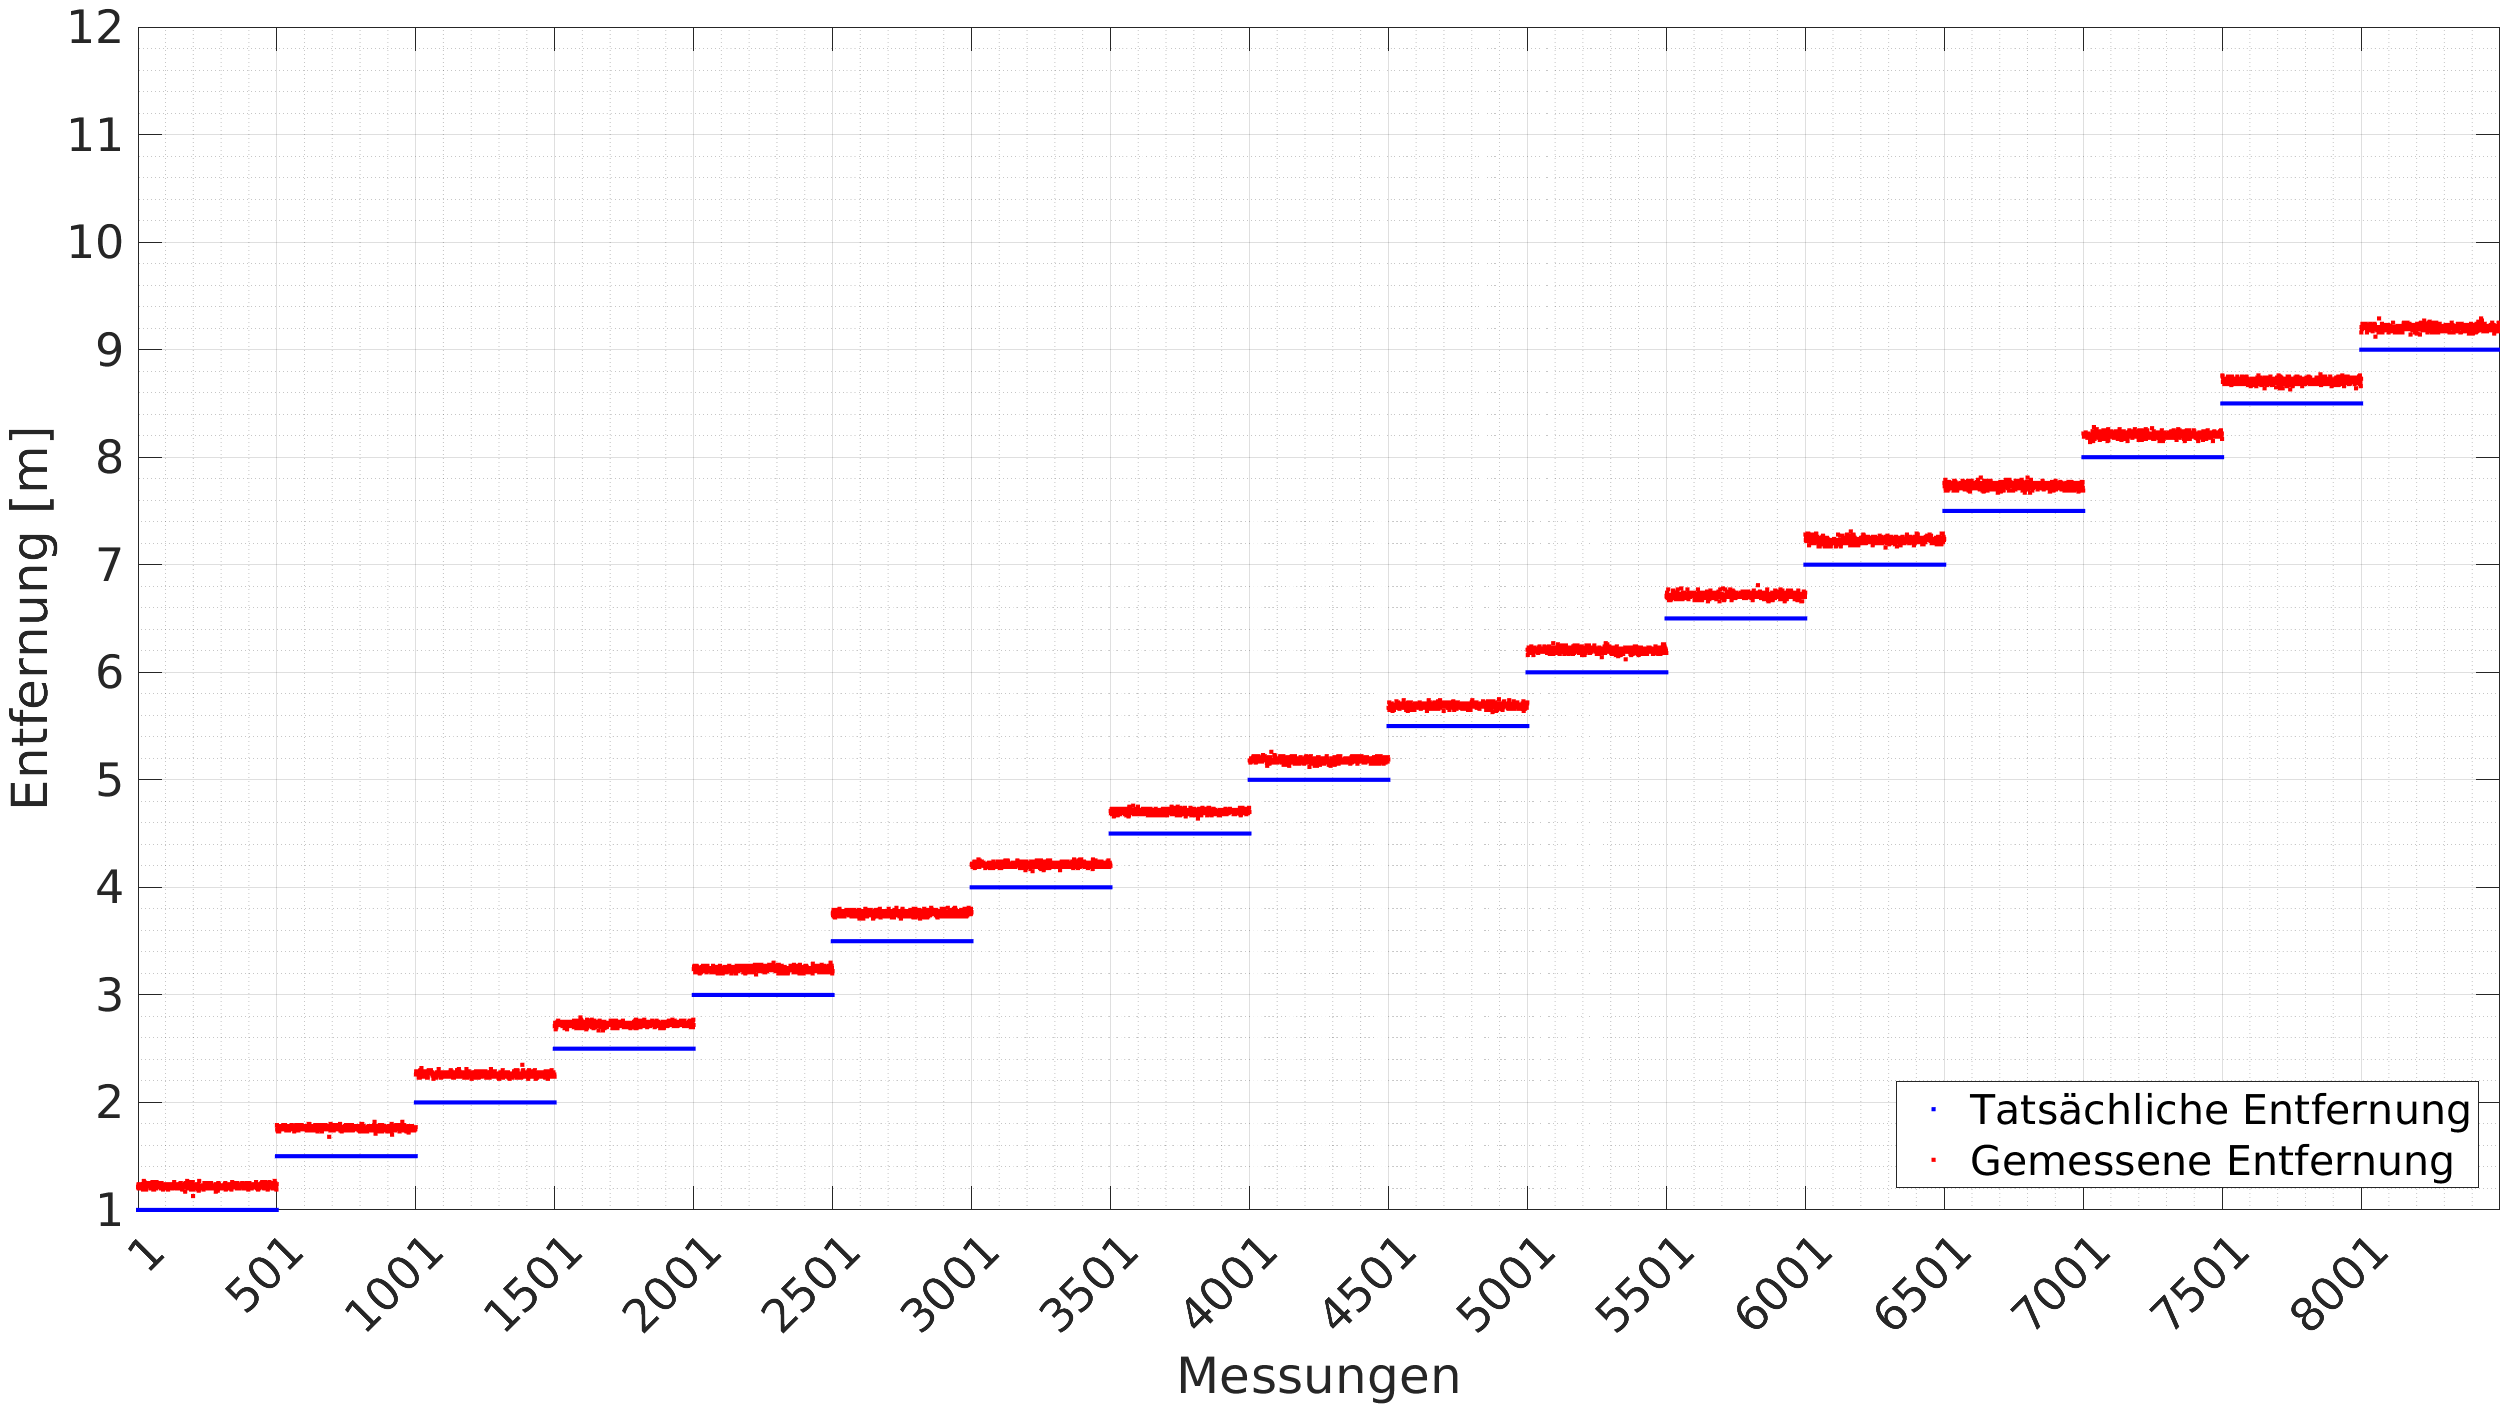
\includegraphics[width=\linewidth]{entfernungsmessung_2018_01_20_los}
		\caption{\glsentryshort{los}}
		\label{fig:entfernungsmessung_2018_01_20_los}
	\end{subfigure}
	\hfill
	\begin{subfigure}[b]{0.49\linewidth}
		\centering
		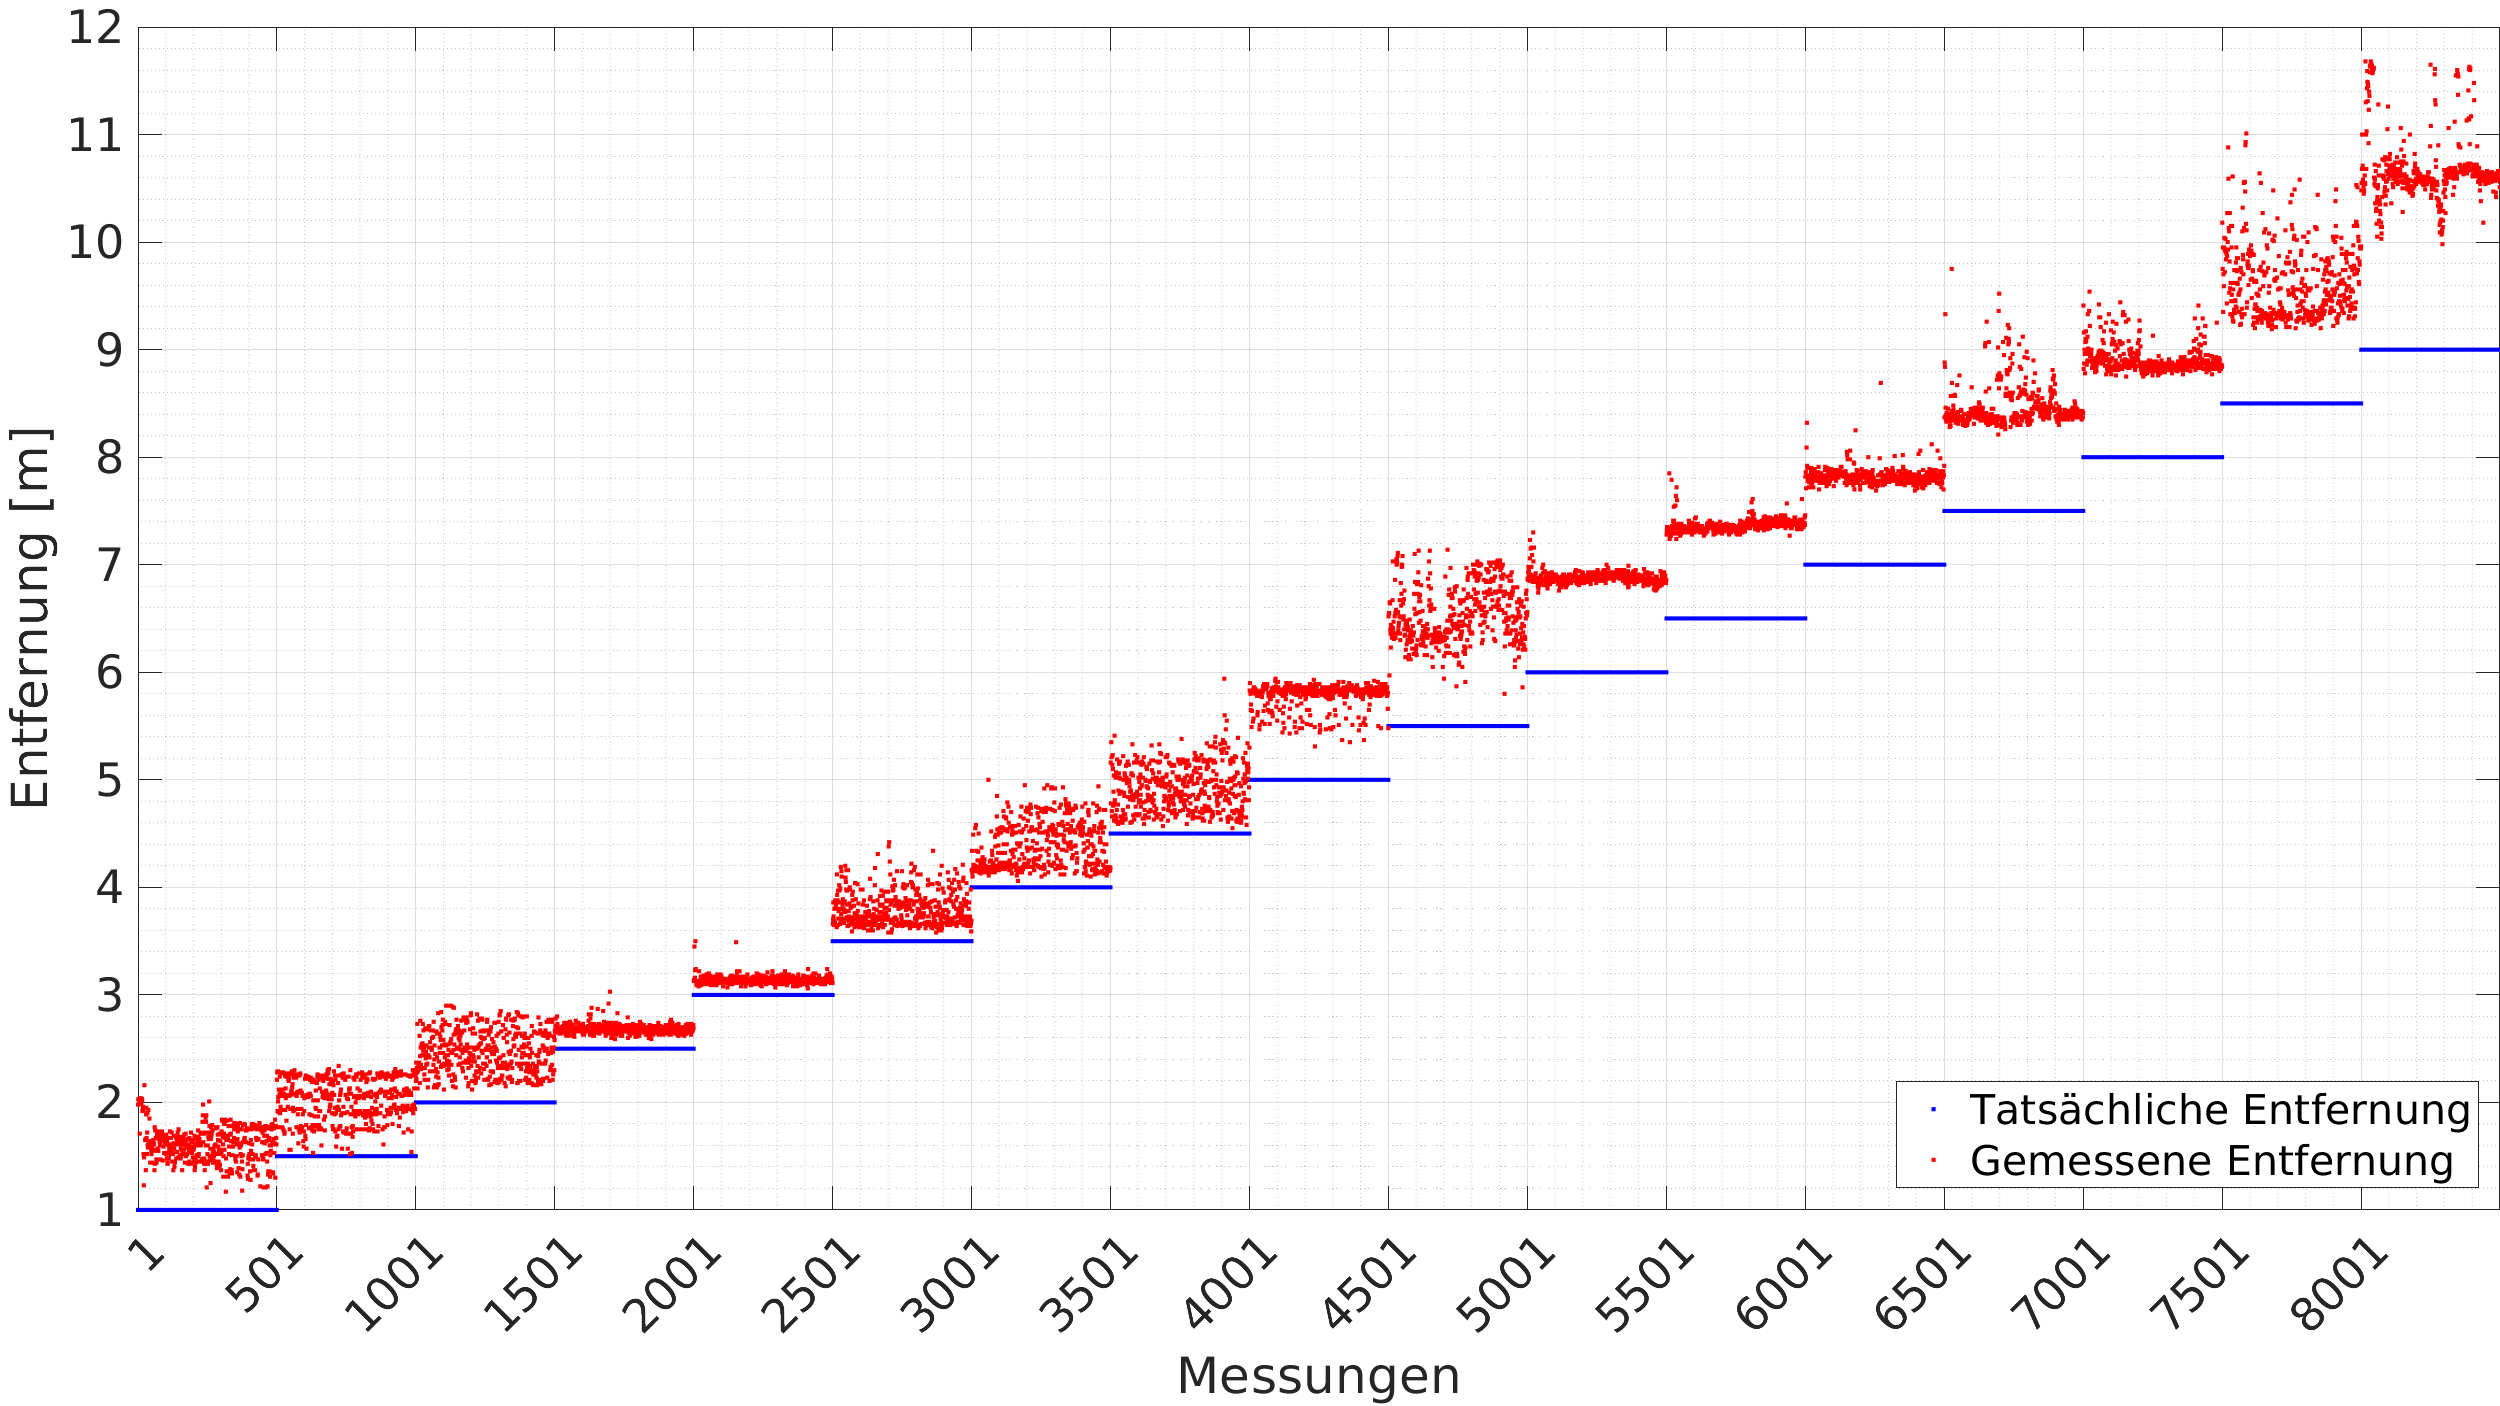
\includegraphics[width=\linewidth]{entfernungsmessung_2018_01_20_nlos_water}
		\caption{\glsentryshort{nlos} mit einem wassergefüllten Kunststoffbehälter.}
		\label{fig:entfernungsmessung_2018_01_20_nlos_water}
	\end{subfigure}
	\par
	\bigskip
	\begin{subfigure}[b]{0.49\linewidth}
		\centering
		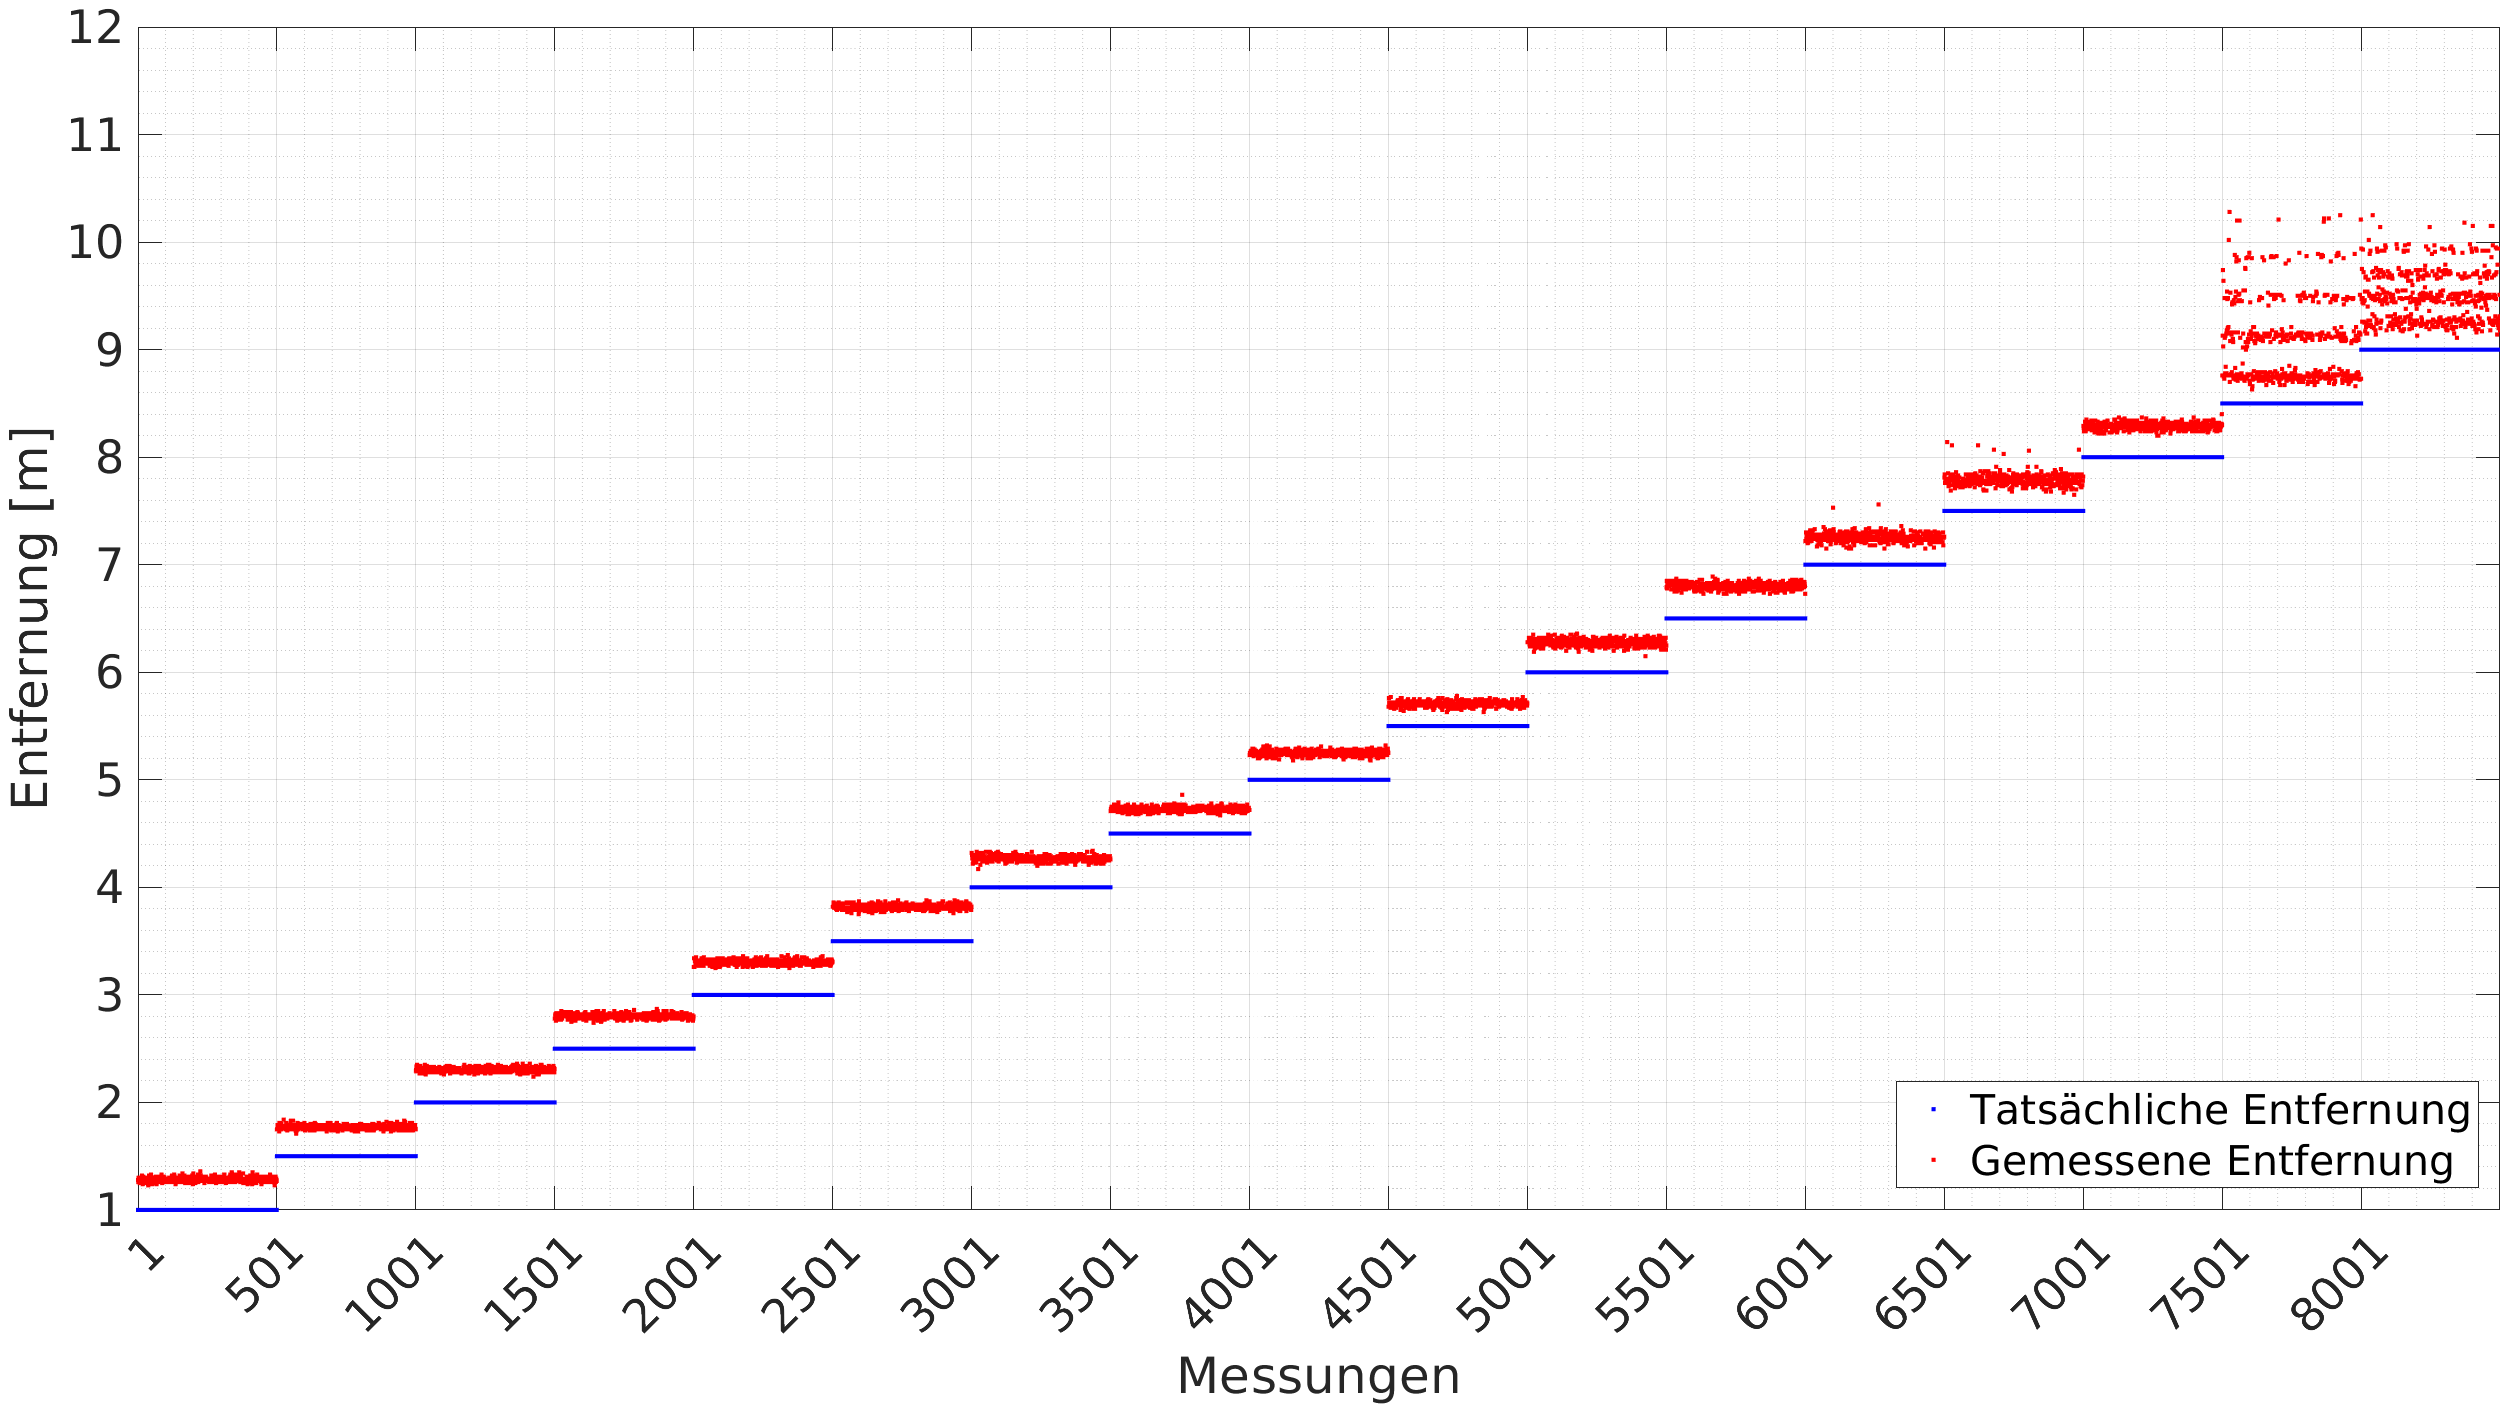
\includegraphics[width=\linewidth]{entfernungsmessung_2018_01_20_nlos_metal}
		\caption{\glsentryshort{nlos} mit einem Aluminiumblech in einer Entfernung von \SI{50}{\centi\meter}.}
		\label{fig:entfernungsmessung_2018_01_20_nlos_metal}
	\end{subfigure}
	\hfill
	\begin{subfigure}[b]{0.49\linewidth}
		\centering
		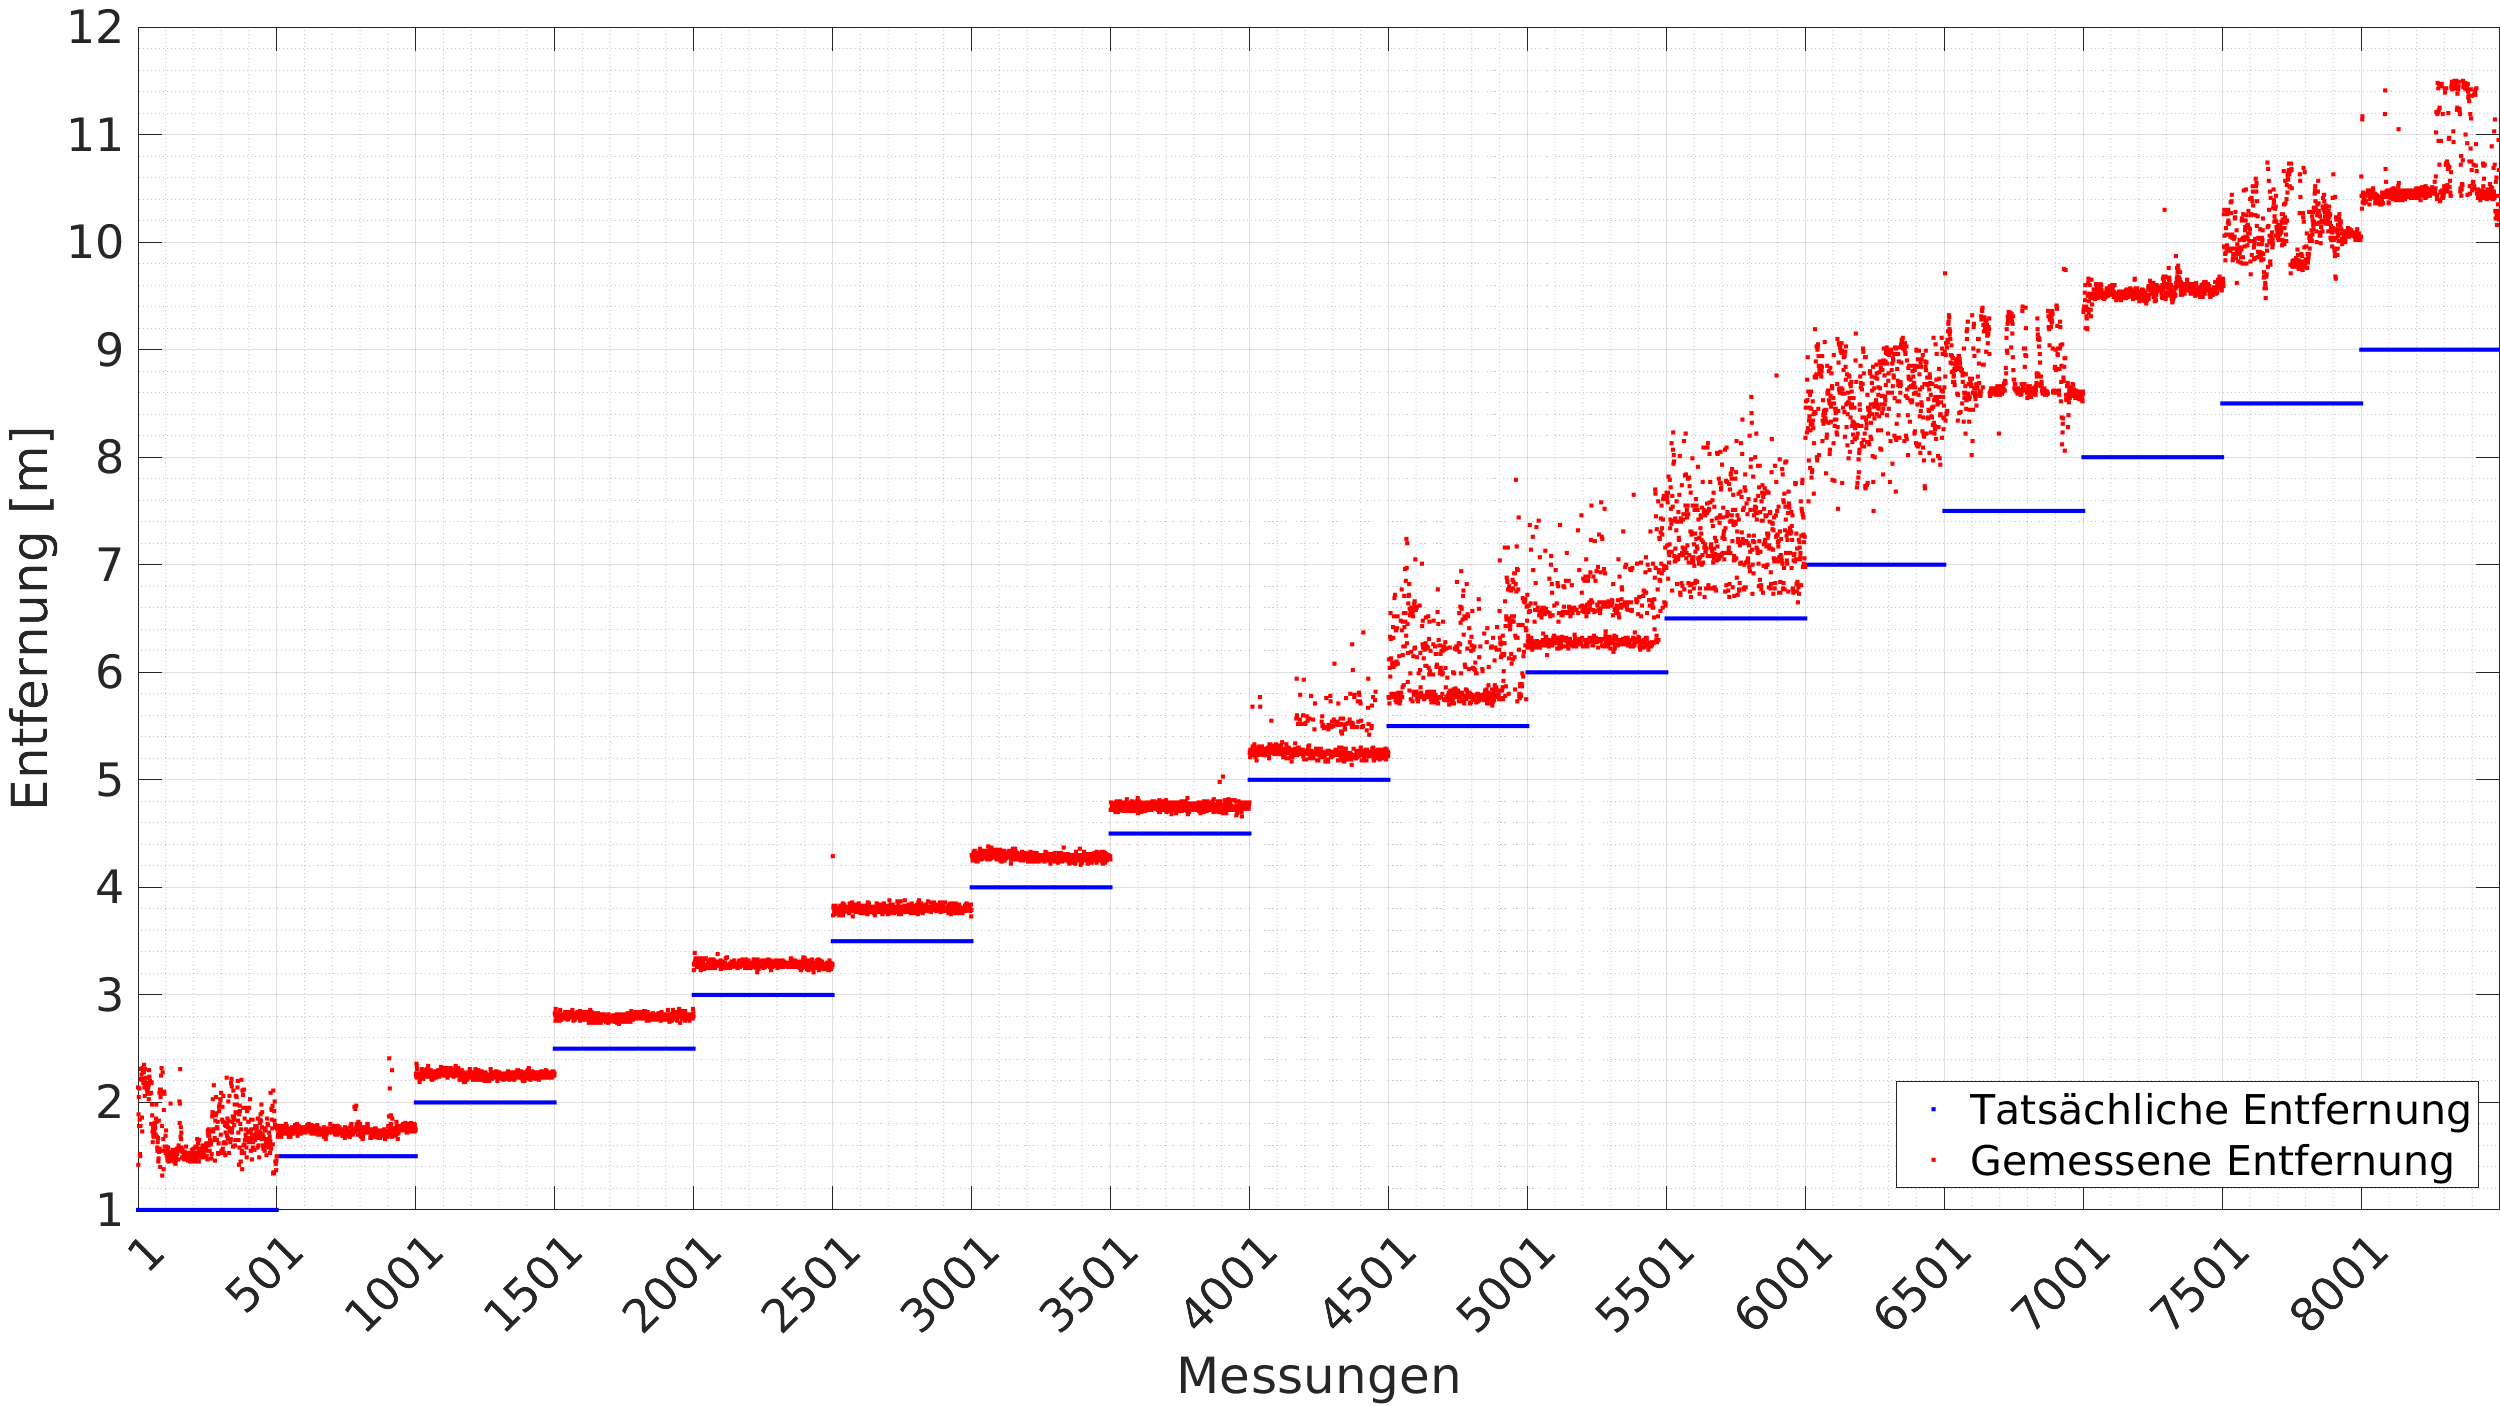
\includegraphics[width=\linewidth]{entfernungsmessung_2018_01_20_nlos_metal2}
		\caption{\glsentryshort{nlos} mit einem Aluminiumblech in einer Entfernung von \SI{5}{\centi\meter}.}
		\label{fig:entfernungsmessung_2018_01_20_nlos_metal2}
	\end{subfigure}
	\caption{Tatsächliche und gemessene \glsentryshort{los}- und \glsentryshort{nlos}-Entfernungen.}
	\label{fig:entfernungsmessung_2018_01_20}
\end{figure}


%%%%%%%%%%%%%%%%%%%%%%%%%%%%%%%%%%%%%%%%%%%%%%%%%%%%%%%%%%%%%%%%%%%%%%%%%%%%%%%%
%
%
%
%%%%%%%%%%
\section{Trajektorie}

Der Softwarearchitektur, siehe \autoref{fig:architektur_grouped}, ist zu entnehmen, dass die Odometriedaten eine wichtige Rolle für den \gls{roslam} spielen. Insgesamt stehen drei Odometriequellen zur Verfügung. Einmal die Inkrementalgeber der Antriebseinheit und zwei laserbasierte Odometrieen. Alle drei Verfahren werden im Folgenden auf ihre Genauigkeit untersucht.

Für die Untersuchung werden zwei Messfahrten durchgeführt. Bei der ersten Messfahrt entspricht die Trajektorie einem abgerundeten Rechteckt und bei der zweiten wird das abgerundete Rechteck um mehrere Kreisbahnen erweitert. In beiden Fällen kehrte die Roboterplattform zu der Startposition zurück um den Versatz berechnen zu können. Im Folgenden wird nur noch die zweite Messfahrt betrachtet, da bei der ersten alle Verfahren in etwa gleich abgeschnitten haben, siehe \autoref{fig:Record_2018-02-08-12-30-43_trajectory}.

Alle \gls{ros}-Nachrichten, der beiden Messfahrten, wurden aufgezeichnet und in separaten Bag-Dateien abgespeichert. Bevor die Bag-Dateien mit den laserbasierten Odometriequellen untersucht werden können, müssen die Odometriedaten der Inkrementalgeber entfernt werden, um widersprüchliche Informationen aus mehreren Odometriequellen zu verhindern. Für die Filterung der Bag-Dateien ist das Kommandozeilenprogramm \textit{rosbag} zuständig. Über den Parameter \textit{filter} und einem Python-Ausdruck werden alle Transformationsnachrichten zwischen dem Roboterplattform- und dem Odometrie-Koordinatensystem entfernt.

Mit dem \gls{rosm} \textit{hector\_trajectory\_server} und dem Skript \textit{trajectory\_to\_csv.py} wurden die Trajektorien der drei Odometriequellen in eine CSV-Datei gespeichert, um diese auswerten zu können. Dabei wurden aus den ungefilterten Aufzeichnungen die Trajektorie der Inkrementalgeber extrahiert. Mit den \glsuseri{rosm} für die laserbasierten Odometrieen und den gefilterten Aufzeichnungen wurden die laserbasierten Trajektorien extrahiert.

Das \gls{rosm} \textit{hector\_trajectory\_server} hat die Möglichkeit, die Trajektorie im Odometrie- und im Karten-Koordinatensystem aufzunehmen. Die Transformation zwischen dem Karten- und dem Roboterplattform-Koordinatensystem wird durch das \gls{rosm} \textit{hector\_mapping} anhand der 2D-Laser-Entfernungsmessung bestimmt. Dadurch eignet es sich ideal, um als Ground Truth Trajektorie verwendet zu werden. Diese Ground Truth Trajektorie wird dann mit den Trajektorien verglichen, die im Odometrie-Koordinatensystem der jeweiligen Odometriequelle aufgezeichnet wurde.

% Um die Trajektorie in einer Karte der Umwelt darzustellen, wird die Belegtheitskarte aus dem \gls{rosm} \textit{hector\_mapping} extrahiert. Das erfolgt mit dem Befehl \textit{rosrun map\_server map\_saver -f file\_name}.

Sowohl die Karte der Umwelt als auch die verfahrenen Trajektorien sind in der \autoref{fig:Record_2018-02-08-12-33-53_trajectory} dargestellt. Die Ground Truth Trajektorie, mit der die anderen Trajektorien verglichen werden, ist in der \autoref{fig:Record_2018-02-08-12-33-53_trajectory1} zu sehen. Deutlich zu erkennen ist, dass die Trajektorie der Inkrementalgeber sowohl in der X- als auch in der Y-Achse gestaucht ist, siehe \autoref{fig:Record_2018-02-08-12-33-53_trajectory2}. Die laserbasierte Odometrie des LSM-Verfahrens hat große Problem mit den gefahrenen Kreisbahnen und driftet zum Ende hin sehr stark von der Startposition ab, siehe \autoref{fig:Record_2018-02-08-12-33-53_trajectory3}. Einzig die laserbasierte Odometrie des \gls{rf2o}-Verfahrens bildet die gefahrene Trajektorie gegenüber dem Ground Turth gut ab, auch wenn die Start- und Zielpositionen voneinander abweichen, siehe \autoref{fig:Record_2018-02-08-12-33-53_trajectory4}.

\begin{figure}
	\centering
	\begin{subfigure}{0.49\linewidth}
		\centering
		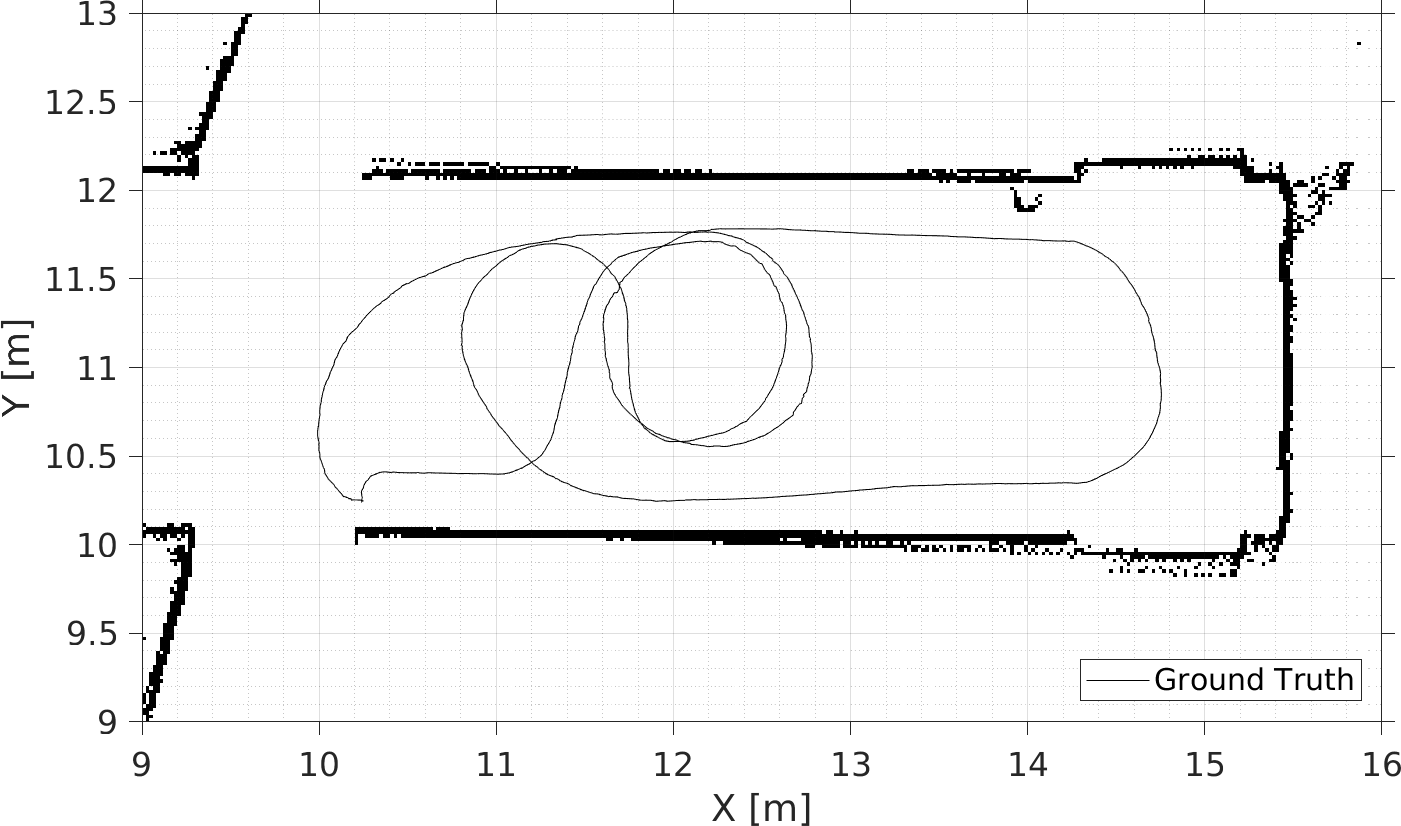
\includegraphics[width=\linewidth]{Record_2018-02-08-12-33-53_trajectory1}
		\caption{Ground Truth}
		\label{fig:Record_2018-02-08-12-33-53_trajectory1}
	\end{subfigure}
	\hfill
	\begin{subfigure}{0.49\linewidth}
		\centering
		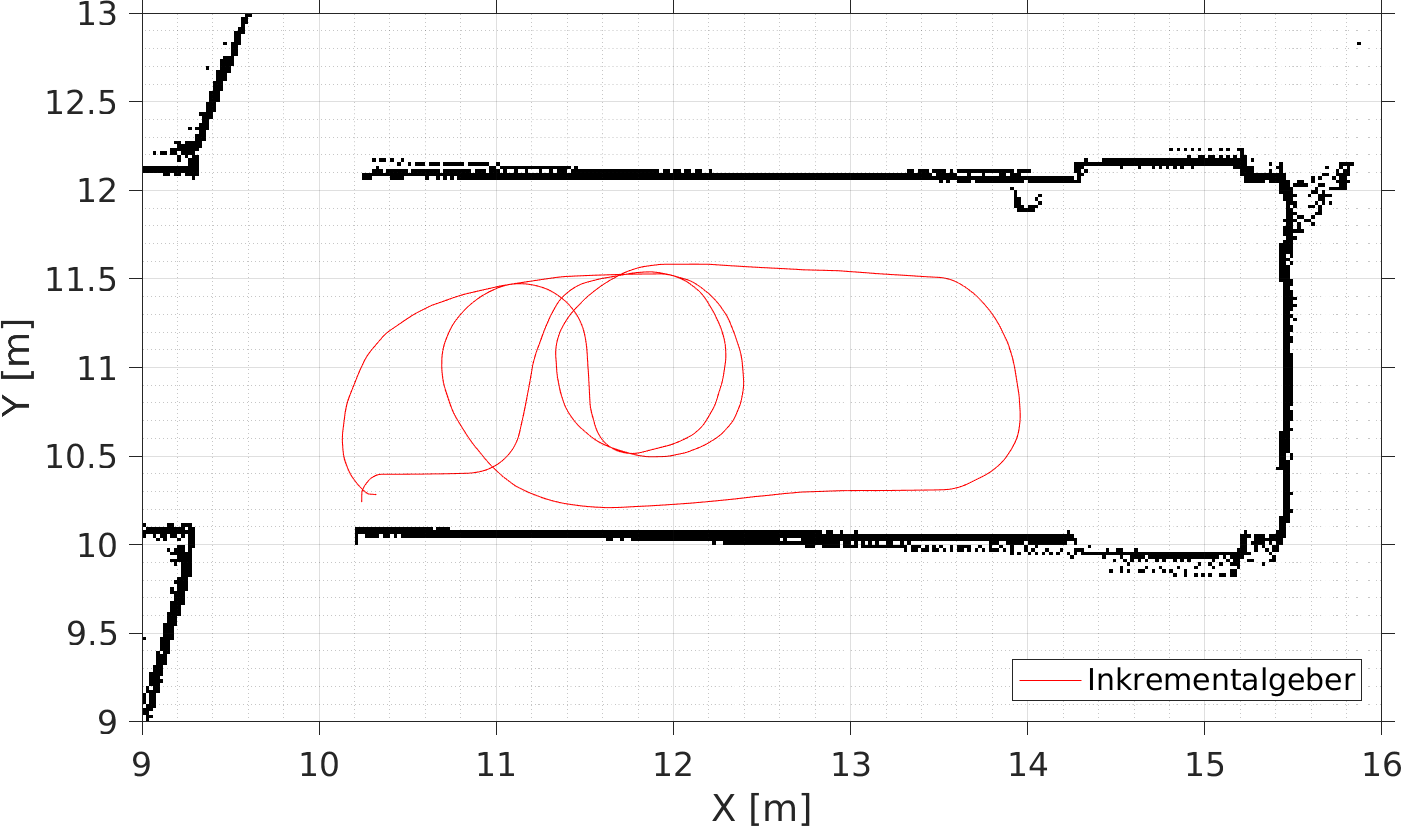
\includegraphics[width=\linewidth]{Record_2018-02-08-12-33-53_trajectory2}
		\caption{Inkrementalgeber}
		\label{fig:Record_2018-02-08-12-33-53_trajectory2}
	\end{subfigure}
	\par
	\bigskip
	\begin{subfigure}{0.49\linewidth}
		\centering
		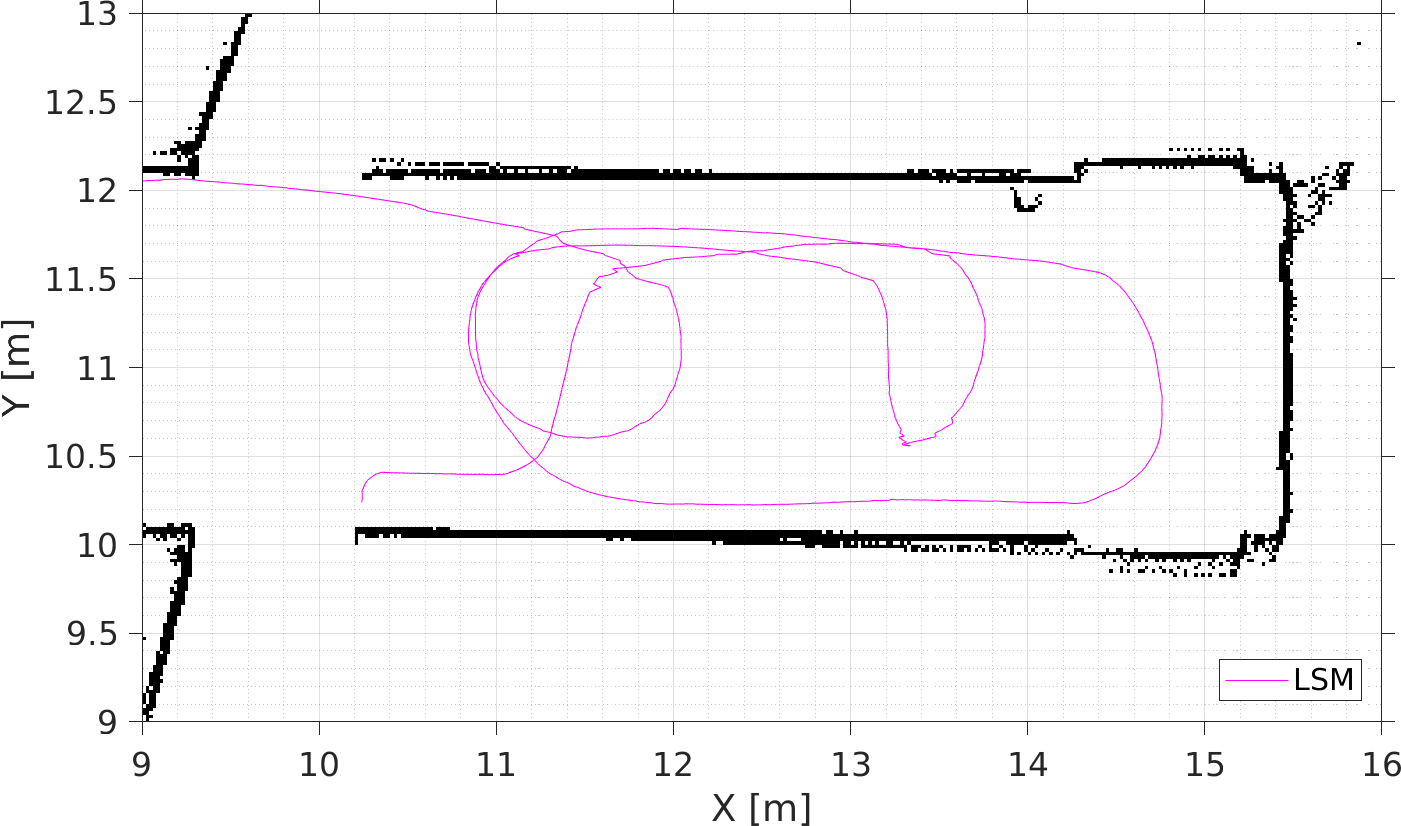
\includegraphics[width=\linewidth]{Record_2018-02-08-12-33-53_trajectory3}
		\caption{LSM}
		\label{fig:Record_2018-02-08-12-33-53_trajectory3}
	\end{subfigure}
	\hfill
	\begin{subfigure}{0.49\linewidth}
		\centering
		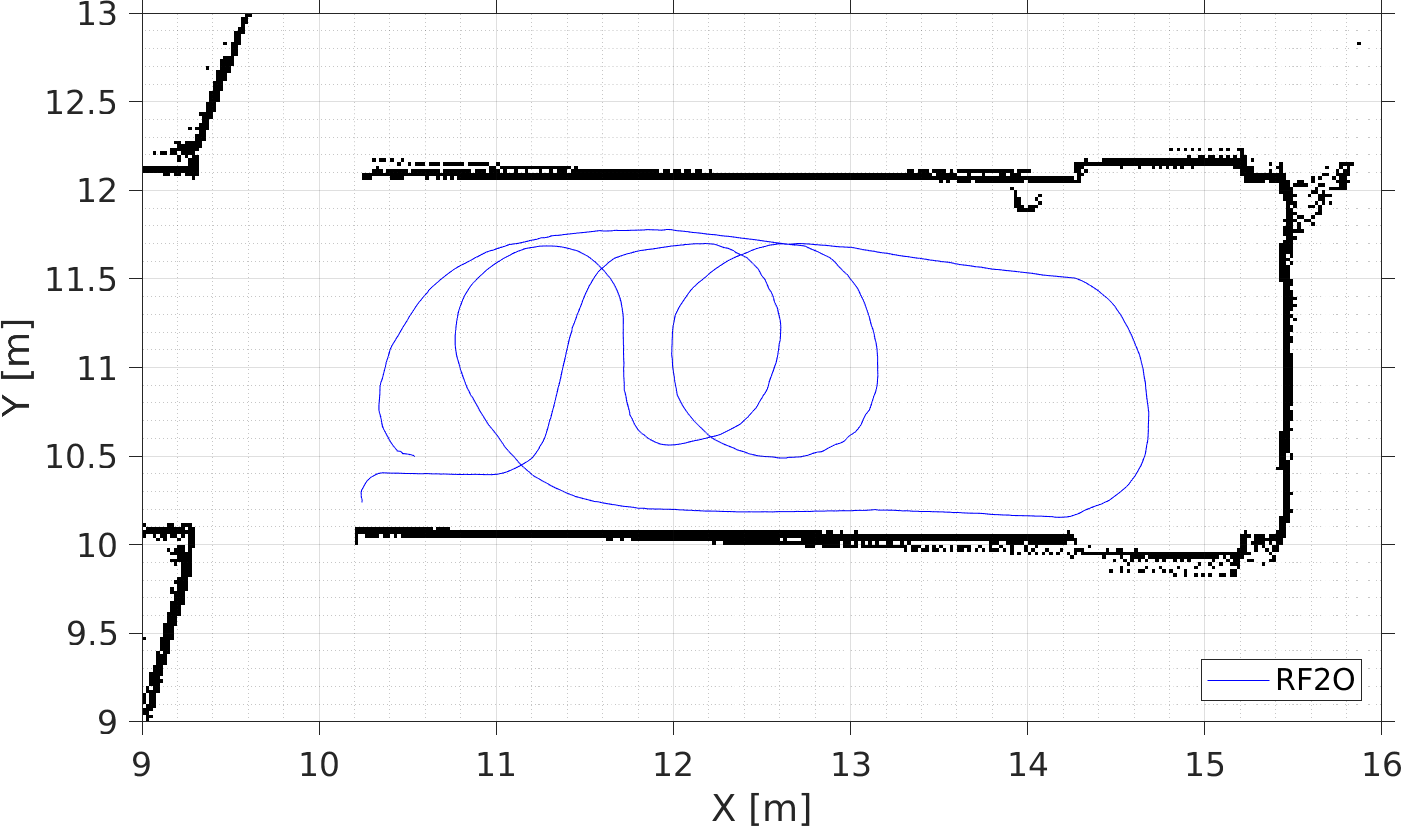
\includegraphics[width=\linewidth]{Record_2018-02-08-12-33-53_trajectory4}
		\caption{RF2O}
		\label{fig:Record_2018-02-08-12-33-53_trajectory4}
	\end{subfigure}
	\caption{Die Trajektorien der verschiedenen Odometriequellen.}
	\label{fig:Record_2018-02-08-12-33-53_trajectory}
\end{figure}

Bei der stochastischen Auswertung war eine direkte zeitliche Zuordnung der Messwerte aller drei Verfahren zum Ground Truth nicht möglich, da jede Odometriequelle eine spezifische Verarbeitungsdauer besitzt. Deshalb wird pro Sekunde der Mittelwert der verfügbaren Positionen gebildet und aus dieser dann die Entfernung zur Ground Truth Position berechnet, siehe \autoref{tab:stochastik_odometrie_quellen}.

Bestätigt wird die visuelle Einschätzung durch die stochastischen Auswertungen der Entfernung der Position zur Ground Truth Position, siehe \autoref{tab:stochastik_odometrie_quellen}. Das LSM-Verfahren weicht im Mittelwert und bei der Standardabweichung deutlich von dem Inkrementalgebern und dem \gls{rf2o}-Verfahren ab. Das der Mittelwert und die Standardabweichung zwischen den Inkrementalgebern und dem \gls{rf2o}-Verfahren nur sehr geringe Unterschiede aufweisen, jedoch große Unterschiede in der visuellen Trajektorie festzustellen sind, kann nur damit erklärt werden, das sich die aufsummierten Fehler der Inkrementalgebern bei der Rückfahrt wieder aufheben.

\begin{table}
	\centering
	\begin{tabular}{||l||c|c|c||c|c||}
		\hline
		Odometriequelle & $\overline{x}$ & $\sigma$ & $SE_{\overline{x}}$ & Min & Max \\
		& [\si{\meter}] & [\si{\meter}] & [\si{\meter}] & [\si{\meter}] & [\si{\meter}] \\
		\hline
		\hline
		Inkrementalgeber & \num{0.327} & \num{0.203} & \num{0.017} & \num{0.000} & \num{0.806} \\
		LSM & \num{0.875} & \num{0.929} & \num{0.079} & \num{0.000} & \num{2.477} \\
		RF2O & \num{0.247} & \num{0.180} & \num{0.015} & \num{0.002} & \num{0.558} \\
		\hline
	\end{tabular}
	\caption{Stochastische Eigenschaften der Entfernungen zwischen der Odometrie- und der Ground Truth Position.}
	\label{tab:stochastik_odometrie_quellen}
\end{table}

Da die Trajektorie des laserbasierten \gls{rf2o}-Verfahren am besten der Ground Truth Trajektorie entspricht, wird diese als Odometriequelle für das \gls{roslam}-Verfahren verwendet.


%%%%%%%%%%%%%%%%%%%%%%%%%%%%%%%%%%%%%%%%%%%%%%%%%%%%%%%%%%%%%%%%%%%%%%%%%%%%%%%%
%
%
%
%%%%%%%%%%
\section{RO-SLAM}


%%%%%%%%%%%%%%%%%%%%%%%%%%%%%%%%%%%%%%%%%%%%%%%%%%%%%%%%%%%%%%%%%%%%%%%%%%%%%%%%
%
%	- Fragen
%		- Wer ist für die Positionsschätzung zuständig? => PF
%		- Welche Datensätze wurden verwendet?
%		- Wie gut ist die Positionsschätzung?
%
%%%%%%%%%%
\subsection{Positionsschätzung}

Im vorherigen Abschnitt wurde bereits die Trajektorie der verschiedenen Odometriequellen untersucht. Die Entscheidung fiel auf das \gls{rf2o}-Verfahren, mit dem nun die Positionsschätzung des \gls{roslam}-Verfahren untersucht wird. Es wird dabei die Trajektorie mit dem abgerundeten Rechteck mit mehrere Kreisbahnen verwendet, siehe \autoref{fig:Record_2018-02-08-12-33-53_trajectory}. Da auch die Entfernungsmessungen der \glspl{uwbm} einen Einfluss auf die Positionsschätzung haben, werden neben den realen auch virtuelle \glsuseri{uwbm} verwendet. Die virtuellen \glspl{uwbm} zeichnen sich dadurch aus, dass ihre Entfernungsmessungen keine Fehler aufweisen und daher als perfekt angesehen werden können.

In der \autoref{fig:Record_2018-02-08-12-33-53_filtered_trajectory_pf} ist die tatsächliche Trajektorie und die des \gls{roslam} Partikel Filters abgebildet. Die oberen zwei Abbildungen verwenden die Entfernungsmessungen der realen \glspl{uwbm} und die unteren zwei Abbildungen die Entfernungsmessung von virtuellen \glspl{uwbm}. Auf der linken Seite befinden sich die Positionsschätzungen die die Ground Truth Trajektorie gut abbilden und auf der rechten Seite die die sie schlecht abbilden. Während bei den realen \glsuseri{uwbm} die Positionsschätzung sehr große Abweichungen von der Ground Truth Trajektorie besitzt, bildet die Positionsschätzung der virtuellen \glspl{uwbm} die Ground Truth Trajektorie deutlich besser ab, selbst bei der schlechten Abbildung weist die Positionsschätzung nur einen leichten Winkelfehler auf.

Das führt zu der Vermutung, dass die Qualität der Entfernungsmessung einen entscheidenden Einfluss auf die Positionsschätzung des \gls{roslam}-Verfahrens besitzt. Je geringe die Abweichungen der Entfernungsmessung von der tatsächlichen Entfernung desto besser. Bemerkenswert ist es auch, dass die Reproduzierbarkeit der Ergebnisse mit den virtuellen \glsuseri{uwbm} deutlich eher gegeben war, als mit den realen \glsuseri{uwbm}.

% pose_diff.m -> viz_trajectory(...)
\begin{figure}
	\centering
	\begin{subfigure}{0.49\linewidth}
		\centering
		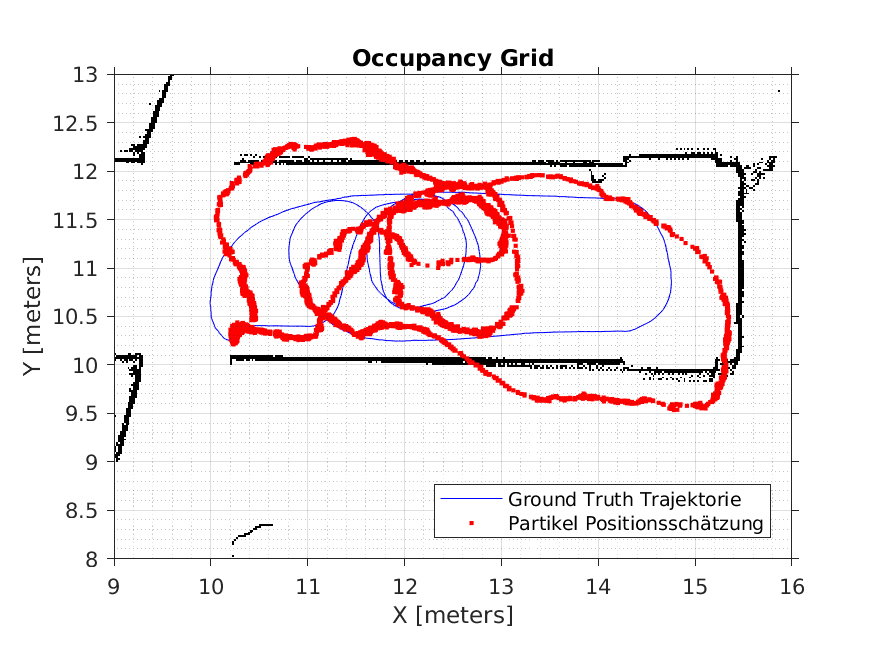
\includegraphics[width=\linewidth]{Record_2018-02-08-12-33-53_filtered_3_trajectory_pf}
		\caption{\textit{Gute} Trajektorie mit den realen \glsuseri{uwbm}.}
		\label{fig:Record_2018-02-08-12-33-53_filtered_3_trajectory_pf}
	\end{subfigure}
	\hfill
	\begin{subfigure}{0.49\linewidth}
		\centering
		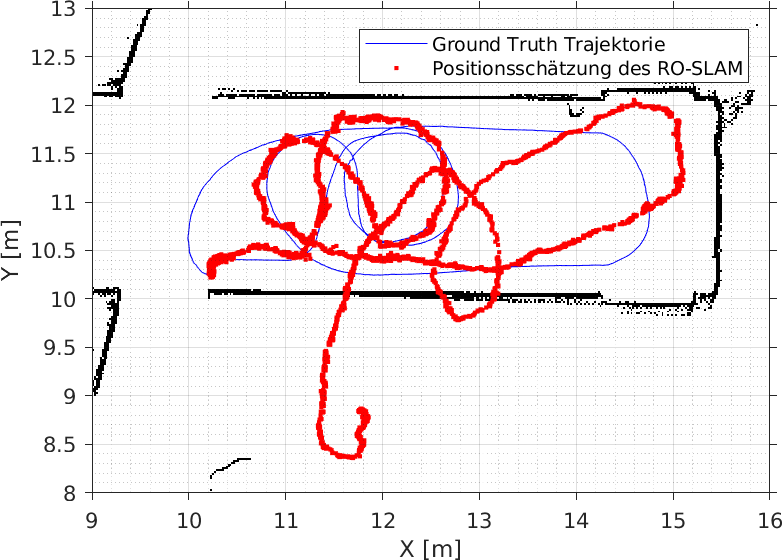
\includegraphics[width=\linewidth]{Record_2018-02-08-12-33-53_filtered_1_trajectory_pf}
		\caption{\textit{Schlechte} Trajektorie mit den realen \glsuseri{uwbm}.}
		\label{fig:Record_2018-02-08-12-33-53_filtered_1_trajectory_pf}
	\end{subfigure}
	\par
	\bigskip
	\begin{subfigure}{0.49\linewidth}
		\centering
		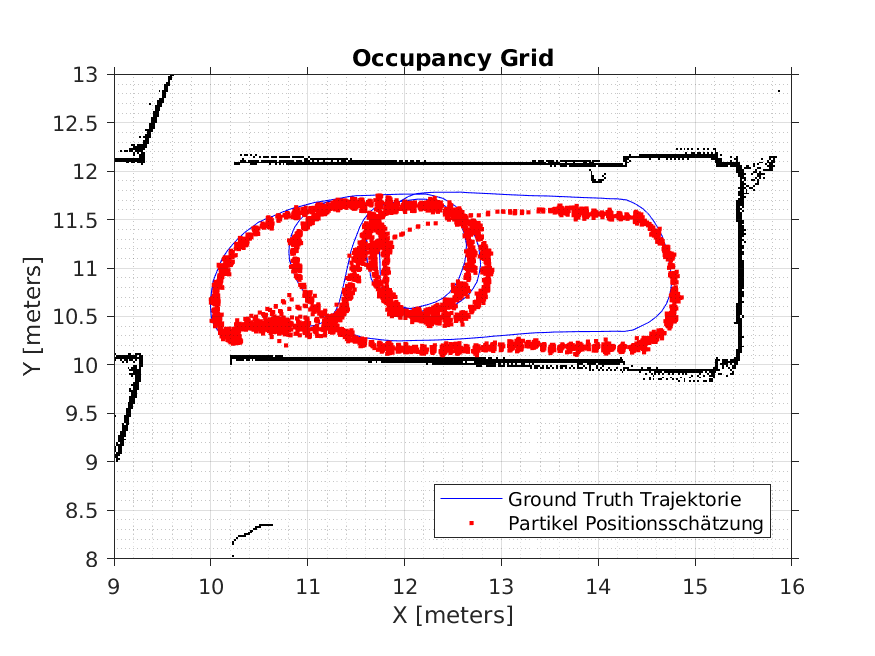
\includegraphics[width=\linewidth]{Record_2018-02-08-12-33-53_filtered_5_trajectory_pf}
		\caption{\textit{Gute} Trajektorie mit den virtuellen \glsuseri{uwbm}.}
		\label{fig:Record_2018-02-08-12-33-53_filtered_5_trajectory_pf}
	\end{subfigure}
	\hfill
	\begin{subfigure}{0.49\linewidth}
		\centering
		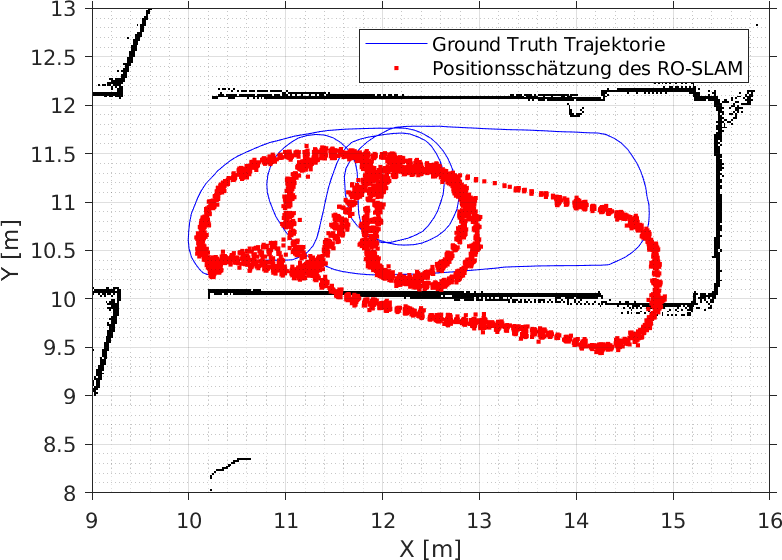
\includegraphics[width=\linewidth]{Record_2018-02-08-12-33-53_filtered_4_trajectory_pf}
		\caption{\textit{Schlechte} Trajektorie mit den virtuellen \glsuseri{uwbm}.}
		\label{fig:Record_2018-02-08-12-33-53_filtered_4_trajectory_pf}
	\end{subfigure}
	\caption{Resultierende Trajektorie aus der Positionsschätzung des \glsentryshort{roslam} mit realen und virtuellen \glsuseri{uwbm}.}
	\label{fig:Record_2018-02-08-12-33-53_filtered_trajectory_pf}
\end{figure}


%%%%%%%%%%%%%%%%%%%%%%%%%%%%%%%%%%%%%%%%%%%%%%%%%%%%%%%%%%%%%%%%%%%%%%%%%%%%%%%%
%
%
%
%%%%%%%%%%
\subsection{Positionsschätzung der \glsentrytext{uwbm}e}

Mit den gleichen Datensätzen wie in \autoref{fig:Record_2018-02-08-12-33-53_filtered_trajectory_pf} wurden nun in der \autoref{fig:Record_2018-02-08-12-33-53_filtered_beacon_error} die Fehlerellipsen für die \glspl{uwbm} eingezeichnet. Um die Fehlerellipsen darstellen zu können, wurde diese mit einem Faktor von 10 skaliert. Die Ground Truth Position der \gls{uwbm} ist an dem schwarzen Kreuz erkennbar. Die Roboterplattform wird durch einen blauen Stern symbolisiert, der sich zu unterschiedlichen Zeitpunkten auf der Trajektorie befindet. Die gepunkteten Linien ordnen der Roboterplattform, zu einem bestimmten Zeitpunkt, die Positionsschätzung der \glspl{uwbm} zu.

Sowohl mit den realen als auch mit den virtuellen \glsuseri{uwbm} verringert sich die Unsicherheit der Positionsschätzung der \glspl{uwbm} kontinuiertlich über die Zeit. Durch die ungenaue Positionsschätzung der Roboterplattform durch die realen \glspl{uwbm} sind auch die Positionsschätzungen der \gls{uwbm} entsprechend verschoben im Bezug zu ihren Ground Truth Position, siehe \autoref{fig:Record_2018-02-08-12-33-53_filtered_3_beacon_error} und \autoref{fig:Record_2018-02-08-12-33-53_filtered_1_beacon_error}. Besser verhält es sich bei den virtuellen \glsuseri{uwbm}, hier entspricht die Positionsschätzung der \glspl{uwbm} dem der Ground Truth Position, siehe \autoref{fig:Record_2018-02-08-12-33-53_filtered_5_beacon_error}. Der Winkelfehler in der Positionsschätzung aus der \autoref{fig:Record_2018-02-08-12-33-53_filtered_4_trajectory_pf} spiegelt sich ebenfalls in der Positionsschätzung der \glspl{uwbm} wieder, siehe \autoref{fig:Record_2018-02-08-12-33-53_filtered_beacon_error}.

% viz_bor_mean_cov, cov=cov*10
\begin{figure}
	\centering
	\begin{subfigure}{0.49\linewidth}
		\centering
		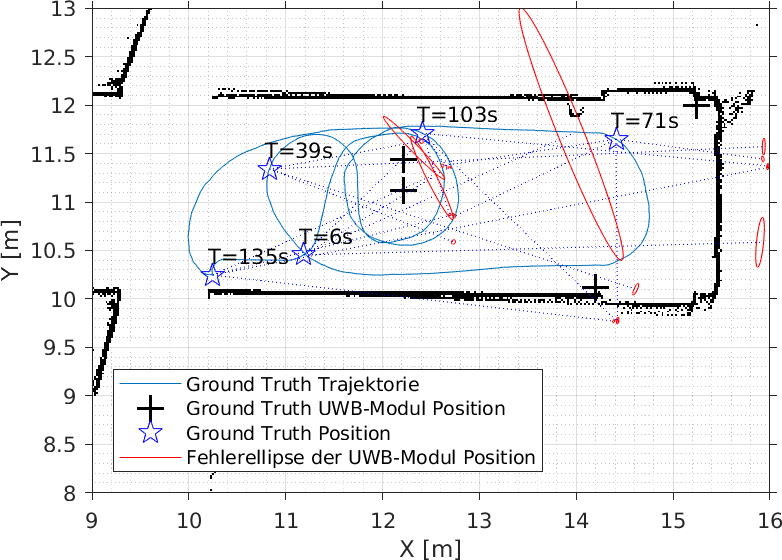
\includegraphics[width=\linewidth]{Record_2018-02-08-12-33-53_filtered_3_beacon_error}
		\caption{Reale \glsentrytext{uwbm}e}
		\label{fig:Record_2018-02-08-12-33-53_filtered_3_beacon_error}
	\end{subfigure}
	\hfill
	\begin{subfigure}{0.49\linewidth}
		\centering
		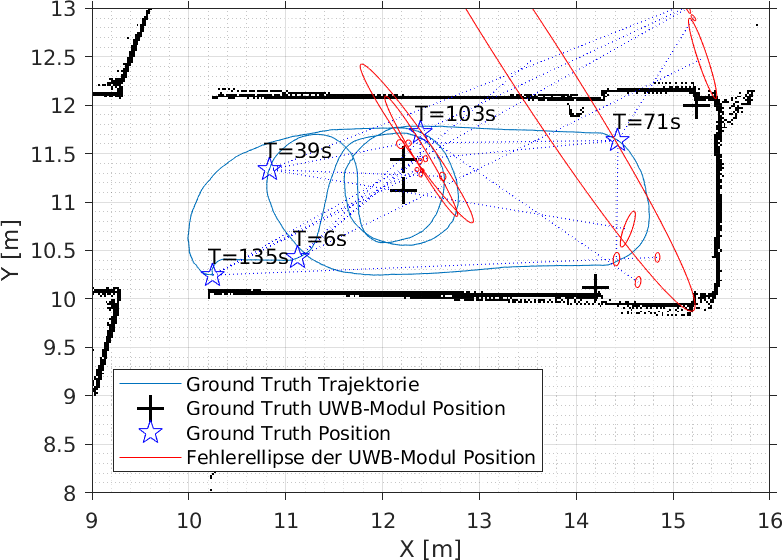
\includegraphics[width=\linewidth]{Record_2018-02-08-12-33-53_filtered_1_beacon_error}
		\caption{Reale \glsentrytext{uwbm}e}
		\label{fig:Record_2018-02-08-12-33-53_filtered_1_beacon_error}
	\end{subfigure}
	\par
	\bigskip
	\begin{subfigure}{0.49\linewidth}
		\centering
		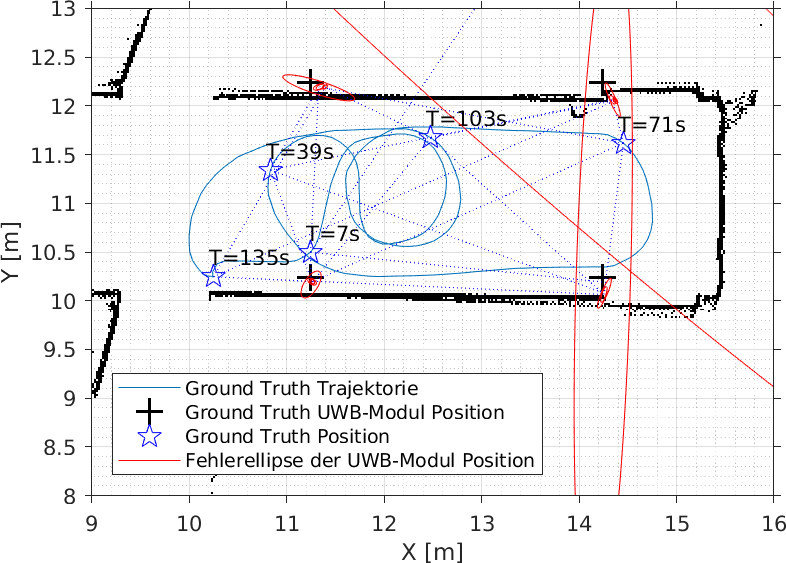
\includegraphics[width=\linewidth]{Record_2018-02-08-12-33-53_filtered_5_beacon_error}
		\caption{Virtuelle \glsentrytext{uwbm}e}
		\label{fig:Record_2018-02-08-12-33-53_filtered_5_beacon_error}
	\end{subfigure}
	\hfill
	\begin{subfigure}{0.49\linewidth}
		\centering
		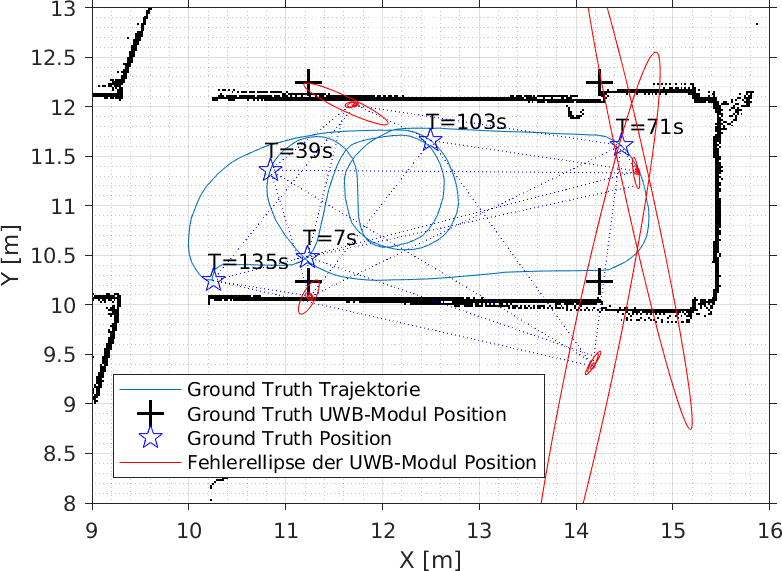
\includegraphics[width=\linewidth]{Record_2018-02-08-12-33-53_filtered_4_beacon_error}
		\caption{Virtuelle \glsentrytext{uwbm}e}
		\label{fig:Record_2018-02-08-12-33-53_filtered_4_beacon_error}
	\end{subfigure}
	\caption{Positionsschätzungen der realen und virtuellen \glsentrytext{uwbm}en zu bestimmten Zeitpunkten.}
	\label{fig:Record_2018-02-08-12-33-53_filtered_beacon_error}
\end{figure}

In den \autoref{tab:distance_between_real_uwb_and_gt} und \autoref{tab:distance_between_virtual_uwb_and_gt} sind die Entfernungen der Positionsschätzung der uwbm zu den Ground Truth Positionen zu bestimten Zeitpunkten aufgelistet. 

Neben einer verbesserung der Positionsschätzung der uwbm ist ebenfalls eine verschlechterung möglich, siehe die Spalten 179 der \autoref{tab:distance_between_real_uwb_and_gt} und Spalte 4 der \autoref{tab:distance_between_virtual_uwb_and_gt}.

Anzumerken ist noch folgendes, das roslam-Verfahren geht von der Annahme aus das die Position der uwbm sich über die Zeit nicht ändert. Während der Auswertung der Daten konnte aber mehrfach beobachtet werden, das sich die positionen der uwbm über die Zeit änderten. Somit ist nicht ausgeschlossen, dass die positionsänderungen der uwbm verfolgt werden kann, sobald die wdf durch das ekf-Verfahren repräsentiert wird.

\begin{table}
	\centering
	\begin{tabular}{||r||c|c|c|c||c|c|c|c||}
		\hline
 & 177 & 178 & 179 & 180 & 177 & 178 & 179 & 180 \\
\hline
\SI{6}{\second} & \SI{0.317}{\meter} & \SI{0.159}{\meter} & \SI{1.561}{\meter} & \SI{1.601}{\meter} & \SI{0.396}{\meter} & \SI{0.212}{\meter} & \SI{0.488}{\meter} & \SI{2.439}{\meter} \\
\SI{39}{\second} & \SI{0.739}{\meter} & \SI{0.261}{\meter} & \SI{0.816}{\meter} & \SI{0.414}{\meter} & \SI{0.426}{\meter} & \SI{0.162}{\meter} & \SI{1.049}{\meter} & \SI{0.687}{\meter} \\
\SI{71}{\second} & \SI{0.584}{\meter} & \SI{0.404}{\meter} & \SI{0.883}{\meter} & \SI{0.406}{\meter} & \SI{0.396}{\meter} & \SI{0.175}{\meter} & \SI{0.905}{\meter} & \SI{0.360}{\meter} \\
\SI{103}{\second} & \SI{0.536}{\meter} & \SI{0.460}{\meter} & \SI{0.972}{\meter} & \SI{0.424}{\meter} & \SI{0.240}{\meter} & \SI{0.167}{\meter} & \SI{1.046}{\meter} & \SI{0.441}{\meter} \\
\SI{135}{\second} & \SI{0.567}{\meter} & \SI{0.490}{\meter} & \SI{0.975}{\meter} & \SI{0.396}{\meter} & \SI{0.281}{\meter} & \SI{0.170}{\meter} & \SI{1.036}{\meter} & \SI{0.709}{\meter} \\
\hline
	\end{tabular}
	\caption{Entfernung der Positionsschätzung der realen \glsentrytext{uwbm} zu den Ground Truth Positionen.}
	\label{tab:distance_between_real_uwb_and_gt}
\end{table}

\begin{table}
	\centering
	\begin{tabular}{||r||c|c|c|c||c|c|c|c||}
		\hline
 & 1 & 2 & 3 & 4 & 1 & 2 & 3 & 4 \\
\hline
\SI{7}{\second} & \SI{0.074}{\meter} & \SI{0.049}{\meter} & \SI{1.572}{\meter} & \SI{0.102}{\meter} & \SI{0.161}{\meter} & \SI{0.756}{\meter} & \SI{1.106}{\meter} & \SI{0.438}{\meter} \\
\SI{39}{\second} & \SI{0.049}{\meter} & \SI{0.165}{\meter} & \SI{0.205}{\meter} & \SI{0.100}{\meter} & \SI{0.156}{\meter} & \SI{0.828}{\meter} & \SI{0.986}{\meter} & \SI{0.486}{\meter} \\
\SI{71}{\second} & \SI{0.050}{\meter} & \SI{0.177}{\meter} & \SI{0.205}{\meter} & \SI{0.108}{\meter} & \SI{0.162}{\meter} & \SI{0.829}{\meter} & \SI{0.956}{\meter} & \SI{0.491}{\meter} \\
\SI{103}{\second} & \SI{0.050}{\meter} & \SI{0.177}{\meter} & \SI{0.226}{\meter} & \SI{0.158}{\meter} & \SI{0.153}{\meter} & \SI{0.861}{\meter} & \SI{0.976}{\meter} & \SI{0.528}{\meter} \\
\SI{135}{\second} & \SI{0.051}{\meter} & \SI{0.177}{\meter} & \SI{0.228}{\meter} & \SI{0.159}{\meter} & \SI{0.154}{\meter} & \SI{0.861}{\meter} & \SI{0.976}{\meter} & \SI{0.529}{\meter} \\
\hline
	\end{tabular}
	\caption{Entfernung der Positionsschätzung der virtuellen \glsentrytext{uwbm} zu den Ground Truth Positionen.}
	\label{tab:distance_between_virtual_uwb_and_gt}
\end{table}

% Wandernde Beacon
% Tabelle mit den Beaconschätzungen (Zeit{0-100%}, Entfernung, usw.)

%%%%%%%%%%%%%%%%%%%%%%%%%%%%%%%%%%%%%%%%%%%%%%%%%%%%%%%%%%%%%%%%%%%%%%%%%%%%%%%%
%
%	- Fragen
%		- Wie lange dauerte es bei SOG/MC bis diese in eine Normalverteilung umgewandelt werden?
%		- PDF, Wahrscheinlichkeitsdichtefunktion (WDF)
%			- Darstellung der WDF durch eine SOG oder durch einen ringförmigen MC Partikel Filter
%		- Kann man den Schwellwert dafür setzen?
%			- MC ja: MC_maxStdToGauss
%			- SOG nein: Fix auf < 0.10
%		- CBeaconMap::internal_insertObservation
%
%%%%%%%%%%
\subsection{Konvergenz der \glsentryshort{wdf}}

Solange die Positionsschätzung der \gls{uwbm} Mehrdeutigkeiten aufweist, werden als \gls{wdf} das \gls{sog}- oder das \gls{mc}-Verfahren eingesetzt. Liegen keine Mehrdeutigkeiten mehr vor, wird die \gls{wdf} mit dem \gls{ekf}-Verfahren abgebildet. Das bedeutet, das jedes \gls{uwbm} nur noch über die Parameter Mittelwert und Kovarianz beschrieben wird, was zu einer Reduktion der genutzten Ressourcen der Verarbeitungseinheit führt.

In der \autoref{tab:timespan_and_distance_to_switch_to_ekf} sind die Zeitspannen und die zurückgelegte Entfernung der Roboterplattform pro \gls{uwbm} aufgelistet, bis die \gls{wdf} durch das \gls{ekf}-Verfahren abgebildet wird. Sowohl mit den virtuellen als auch mit den realen \gls{uwbm} findet die Umwandlung bereits nach weniger als \SI{1}{\meter} bzw. weniger als \SI{10}{\second} statt. Einzig bei den virtuellen \glsuseri{uwbm} benötigte das \gls{sog}-Verfahren deutlich länger. Im Allgemeinen konvergieren sowohl das \gls{sog}- als auch das \gls{mc}-Verfahren gleich schnell.

% conversion_time.m
\begin{table}
	\centering
	\begin{tabular}{||c|c||c||c|c||}
		\hline
\gls{uwbm} & ID & Verfahren & Zeitspanne [\si{\second}] & Entfernung [\si{\meter}] \\
\hline
% Record_2018-02-08-12-33-53_filtered_3
Real & \num{177} & \gls{sog} & \num{3.8} & \num{0.505} \\
Real & \num{178} & \gls{sog} & \num{4.4} & \num{0.616} \\
Real & \num{179} & \gls{sog} & \num{5.0} & \num{0.708} \\
Real & \num{180} & \gls{sog} & \num{7.0} & \num{1.047} \\
\hline
\hline
% Record_2018-02-08-12-33-53_filtered_7
Real & \num{177} & \gls{mc} & \num{5.6} & \num{0.821} \\
Real & \num{178} & \gls{mc} & \num{8.3} & \num{1.207} \\
Real & \num{179} & \gls{mc} & \num{4.8} & \num{0.670} \\
Real & \num{180} & \gls{mc} & \num{8.0} & \num{1.168} \\
\hline
\hline
% Record_2018-02-08-12-33-53_filtered_5
Virtuell & \num{1} & \gls{sog} & \num{3.0} & \num{0.357} \\
Virtuell & \num{2} & \gls{sog} & \num{10.0} & \num{1.396} \\
Virtuell & \num{3} & \gls{sog} & \num{15.5} & \num{2.245} \\
Virtuell & \num{4} & \gls{sog} & \num{4.5} & \num{0.606} \\
\hline
\hline
% Record_2018-02-08-12-33-53_filtered_6
Virtuell & \num{1} & \gls{mc} & \num{1.0} & \num{0.047} \\
Virtuell & \num{2} & \gls{mc} & \num{6.1} & \num{0.868} \\
Virtuell & \num{3} & \gls{mc} & \num{1.0} & \num{0.047} \\
Virtuell & \num{4} & \gls{mc} & \num{5.5} & \num{0.761} \\
\hline
	\end{tabular}
	\caption{Die Zeitspanne und die zurückgelegte Entfernung der Roboterplattform bis die \gls{wdf} durch das \gls{ekf}-Verfahren abgebildet wird.}
	\label{tab:timespan_and_distance_to_switch_to_ekf}
\end{table}
